\chapter{ベンチマーク}
\label{chap_Results}

\section{環境}

ベンチマークの実行環境を,
Table \ref{table_env} に示す.

\begin{table}[hbtp]
  \begin{center}
    \fontsize{9pt}{10pt}\selectfont
    \caption{Benchmark execution environment}
    \begin{tabular}{cc} \hline
      Component & Type                                                               \rule[0pt]{0pt}{10pt} \\ \hline
      CPU       & AMD Ryzen7 1700 (8Cores/16Threads)                                 \rule[0pt]{0pt}{10pt} \\ 
                & Base Clock 3GHz / Max Boost Clock 3.7GHz                           \rule[0pt]{0pt}{10pt} \\
                & Total L1 Cache: 768KB / Total L2 Cache: 4MB / Total L3 Cache: 16MB \rule[0pt]{0pt}{10pt} \\
      Memory    & DDR4-2666 32GB                                                     \rule[0pt]{0pt}{10pt} \\
      OS        & Ubuntu 16.04 LTS                                                   \rule[0pt]{0pt}{10pt} \\
      Compiler  & gcc version 5.4.0 20160609 (Ubuntu 5.4.0-6ubuntu1~16.04.11)        \rule[0pt]{0pt}{10pt} \\ \hline
    \end{tabular}
    \label{table_env}
  \end{center}
\end{table}


%\section{IpCHashT の測定条件}
\section{各ハッシュテーブルの概要と測定条件}
各ハッシュテーブルの key と value に uint64 型を指定して測定する.
テーブルごとの設定を次に示す.
\leavevmode \newline

%
{\bf std::unordered\_map<uint64,uint64>}
\samepage\newline\indent
C++ の標準ライブラリに収録されているハッシュテーブル.
\leavevmode \newline

%
{\bf sstd::CHashT<uint64,uint64>}
\samepage\newline\indent
``Separate chaining with list head cells''
\footnote{``Separate chaining with linked lists'' がテーブルにポインタしか持たず,
ポインタで接続した先から初めて key-value ペアを持つのに対して,
``Separate chaining with list head cells'' ではテーブルにも key-value ペアを格納する.} の実装の 1 つ.
アルゴリズム比較用のサンプル実装として,
最もシンプルなハッシュテーブルアルゴリズムの 1 つを選択した.
本実装では,
テーブルサイズを $2^k-1\ \ (k=1,2,...)$ とし,ハッシュ値の最下位 $k$ ビットを配列インデックスとする.
全要素数がテーブルサイズを超える場合はリハッシュする.
\leavevmode \newline

%
{\bf sstd::IpCHashT<uint64,uint64> (as uint8 and maxLF50)}
\samepage\newline\indent
提案アルゴリズムの実装の 1 つ.
uint8 により双方向リストを構成する.
Load factor の最大値を 50 \% に制限している.
テーブルサイズを $2^k-1\ \ (k=1,2,...)$ とし,ハッシュ値の最下位 $k$ ビットを配列インデックスとする.
{\rm bench.hpp} 内では別名として {\rm iHashT\_u8h} を定義する.
\leavevmode \newline

%
{\bf sstd::IpCHashT<uint64,uint64> (as uint8 and maxLF100)}
\samepage\newline\indent
提案アルゴリズムの実装の 1 つ.
uint8 により双方向リストを構成する.
Load factor の制限はなく,link 距離が ``${\rm uint8} の最大値 - 1 = 254$'' を超えるか,テーブルが全て埋まるまで要素を挿入する.
テーブルサイズを $2^k-1\ \ (k=1,2,...)$ とし,ハッシュ値の最下位 $k$ ビットを配列インデックスとする.
{\rm bench.hpp} 内では別名として {\rm iHashT\_u8f} を定義する.
\leavevmode \newline

%
{\bf sstd::IpCHashT<uint64,uint64> (as uint16 and maxLF100)}
\samepage\newline\indent
提案アルゴリズムの実装の 1 つ.
uint16 により双方向リストを構成する.
Load factor の制限はなく,link 距離が ``$uint16 の最大値 - 1 = 65534$'' を超えるか,テーブルが全て埋まるまで要素を挿入する.
テーブルサイズを $2^k-1\ \ (k=1,2,...)$ とし,ハッシュ値の最下位 $k$ ビットを配列インデックスとする.
{\rm bench.hpp} 内では別名として {\rm iHashT\_u16} を定義する.
\leavevmode \newline

%
{\bf google::dense\_hash\_map<uint64,uint64>}
\samepage\newline\indent
Quadratic probing の実装の 1 つ.
メモリ効率が高く,探査速度が速い一方,
キーの値の 1 つを空符号に,削除を行う場合は更にもう 1 つのキー値を削除符号として登録する必要がある.
登録された値は,キーとして使用できない.
登録には set\_empty\_key() 関数と set\_deleted\_key() 関数を用いる.
テーブルサイズは $2^k-1\ \ (k=1,2,...)$ であり,ハッシュ値の最下位 $k$ ビットを配列インデックスとしている.
\leavevmode \newline

%
{\bf ska::flat\_hash\_map<uint64,uint64,ska::power\_of\_two\_std\_hash<uint64>>}
\samepage\newline\indent
Robin Hood Hashing の実装の 1 つ.
ska::power\_of\_two\_std\_hash<uint64> オプションにより,
テーブルサイズを $2^k-1\ \ (k=1,2,...)$ としており,ハッシュ値の最下位 $k$ ビットを配列インデックスとしている.
\leavevmode \newline


\section{結果}
ここでは,IpCHashT の双方向リストを uint8 と uint16 により構成した設定と,load factor の最大値を 50 \% に制限した設定に加えて,
要素探査時に successful search を優先する設定と,unsuccessful search を優先する設定についてベンチマークする.
\leavevmode \newline

%
{\bf 最大 Loadfactor}
\samepage\newline\indent
最大 load factor とテーブルサイズの関係をFig. \ref{fig_bench_LF}に示す.
\leavevmode \newline

%
{\bf メモリ使用量}
\samepage\newline\indent
メモリ使用量とテーブルサイズの関係をFig. \ref{fig_bench_memory},\ref{fig_bench_memory_preAlloc}に示す.
\leavevmode \newline

%
{\bf 挿入}
\samepage\newline\indent
挿入速度とテーブルサイズの関係をFig. 
\ref{fig_bench_insert_preAlloc},\ref{fig_bench_insert_wRehash},\ref{fig_bench_insert}に示す.
挿入処理において,hard insertion では find() 関数を用いるが,soft insertion では,find() 関数を用いない.
本ベンチマークでは,soft insertion のみを用いている.
したがって,successful search major option と unuccessful search major option による違いはない.
\leavevmode \newline

%
{\bf 探査}
\samepage\newline\indent
探査速度とテーブルサイズの関係をFig. 
\ref{fig_bench_find_s_sm},\ref{fig_bench_find_us_sm},
\ref{fig_bench_find_s_um},\ref{fig_bench_find_us_um}に示す.
Fig. \ref{fig_bench_find_s_sm},\ref{fig_bench_find_s_um}は,
コンパイル時 IpCHashT に successful search major option を指定した結果,
Fig. \ref{fig_bench_find_us_sm},\ref{fig_bench_find_us_um}は,
コンパイル時 IpCHashT に unsuccessful search major option を指定した結果である.
\leavevmode \newline

%
{\bf 削除}
\samepage\newline\indent
削除速度とテーブルサイズの関係をFig. 
\ref{fig_bench_erase_sm},
\ref{fig_bench_erase_um}に示す.
Fig. \ref{fig_bench_erase_sm}は successful search major option を指定した結果,
Fig. \ref{fig_bench_erase_um}は unsuccessful search major option を指定した結果である.
\leavevmode \newline

%\newpage

% AMD Ryzen7 1700
% Total L1 Cache: 768 KB
% Total L2 Cache:   4 MB
% Total L3 Cache:  16 MB

% key: uint64, value: uint64 -> 16 Byte/element
% 768 KB / 16 [Byte/element]
% = 768*1024 [Byte] / 16 [Byte/element]
% = 786432 [Byte] / 16 [Byte/element]
% = 49152 [element]
% = 4.9x10^4 [element]

% key: uint64, value: uint64 -> 16 Byte/element
% 4 [MB] / 16 [Byte/element]
% = 4*1024*1024 [Byte] / 16 [Byte/element]
% = (1/4) * 1024*1024 [element]
% = 256*1024 [element]
% = 262144 [element]
% = 2.6x10^5 [element]

% key: uint64, value: uint64 -> 16 Byte/element
% 16 [MB] / 16 [Byte/element]
% = 16*1024*1024 [Byte] / 16 [Byte/element]
% = 1024*1024 [element]
% = 1048576 [element]
% = 1.0x10^6 [element]

%%%%%%%%%%%%%%%%%%%%%%%%%%%%%%%%%%%%%%%%%%%%%%%%%%%%%%%%%%%%%%%%%%%%%%%%%%%%%%%%%%%%%%%%%%%%%%%%%%%%%%%%%%%%%%%%%%%%%%%%%%%%%%%%%%%%%%%%%%%%%%%%%

\newpage
\begin{figure}[]
%\begin{figure}[b]
%  \vspace{-0mm}
  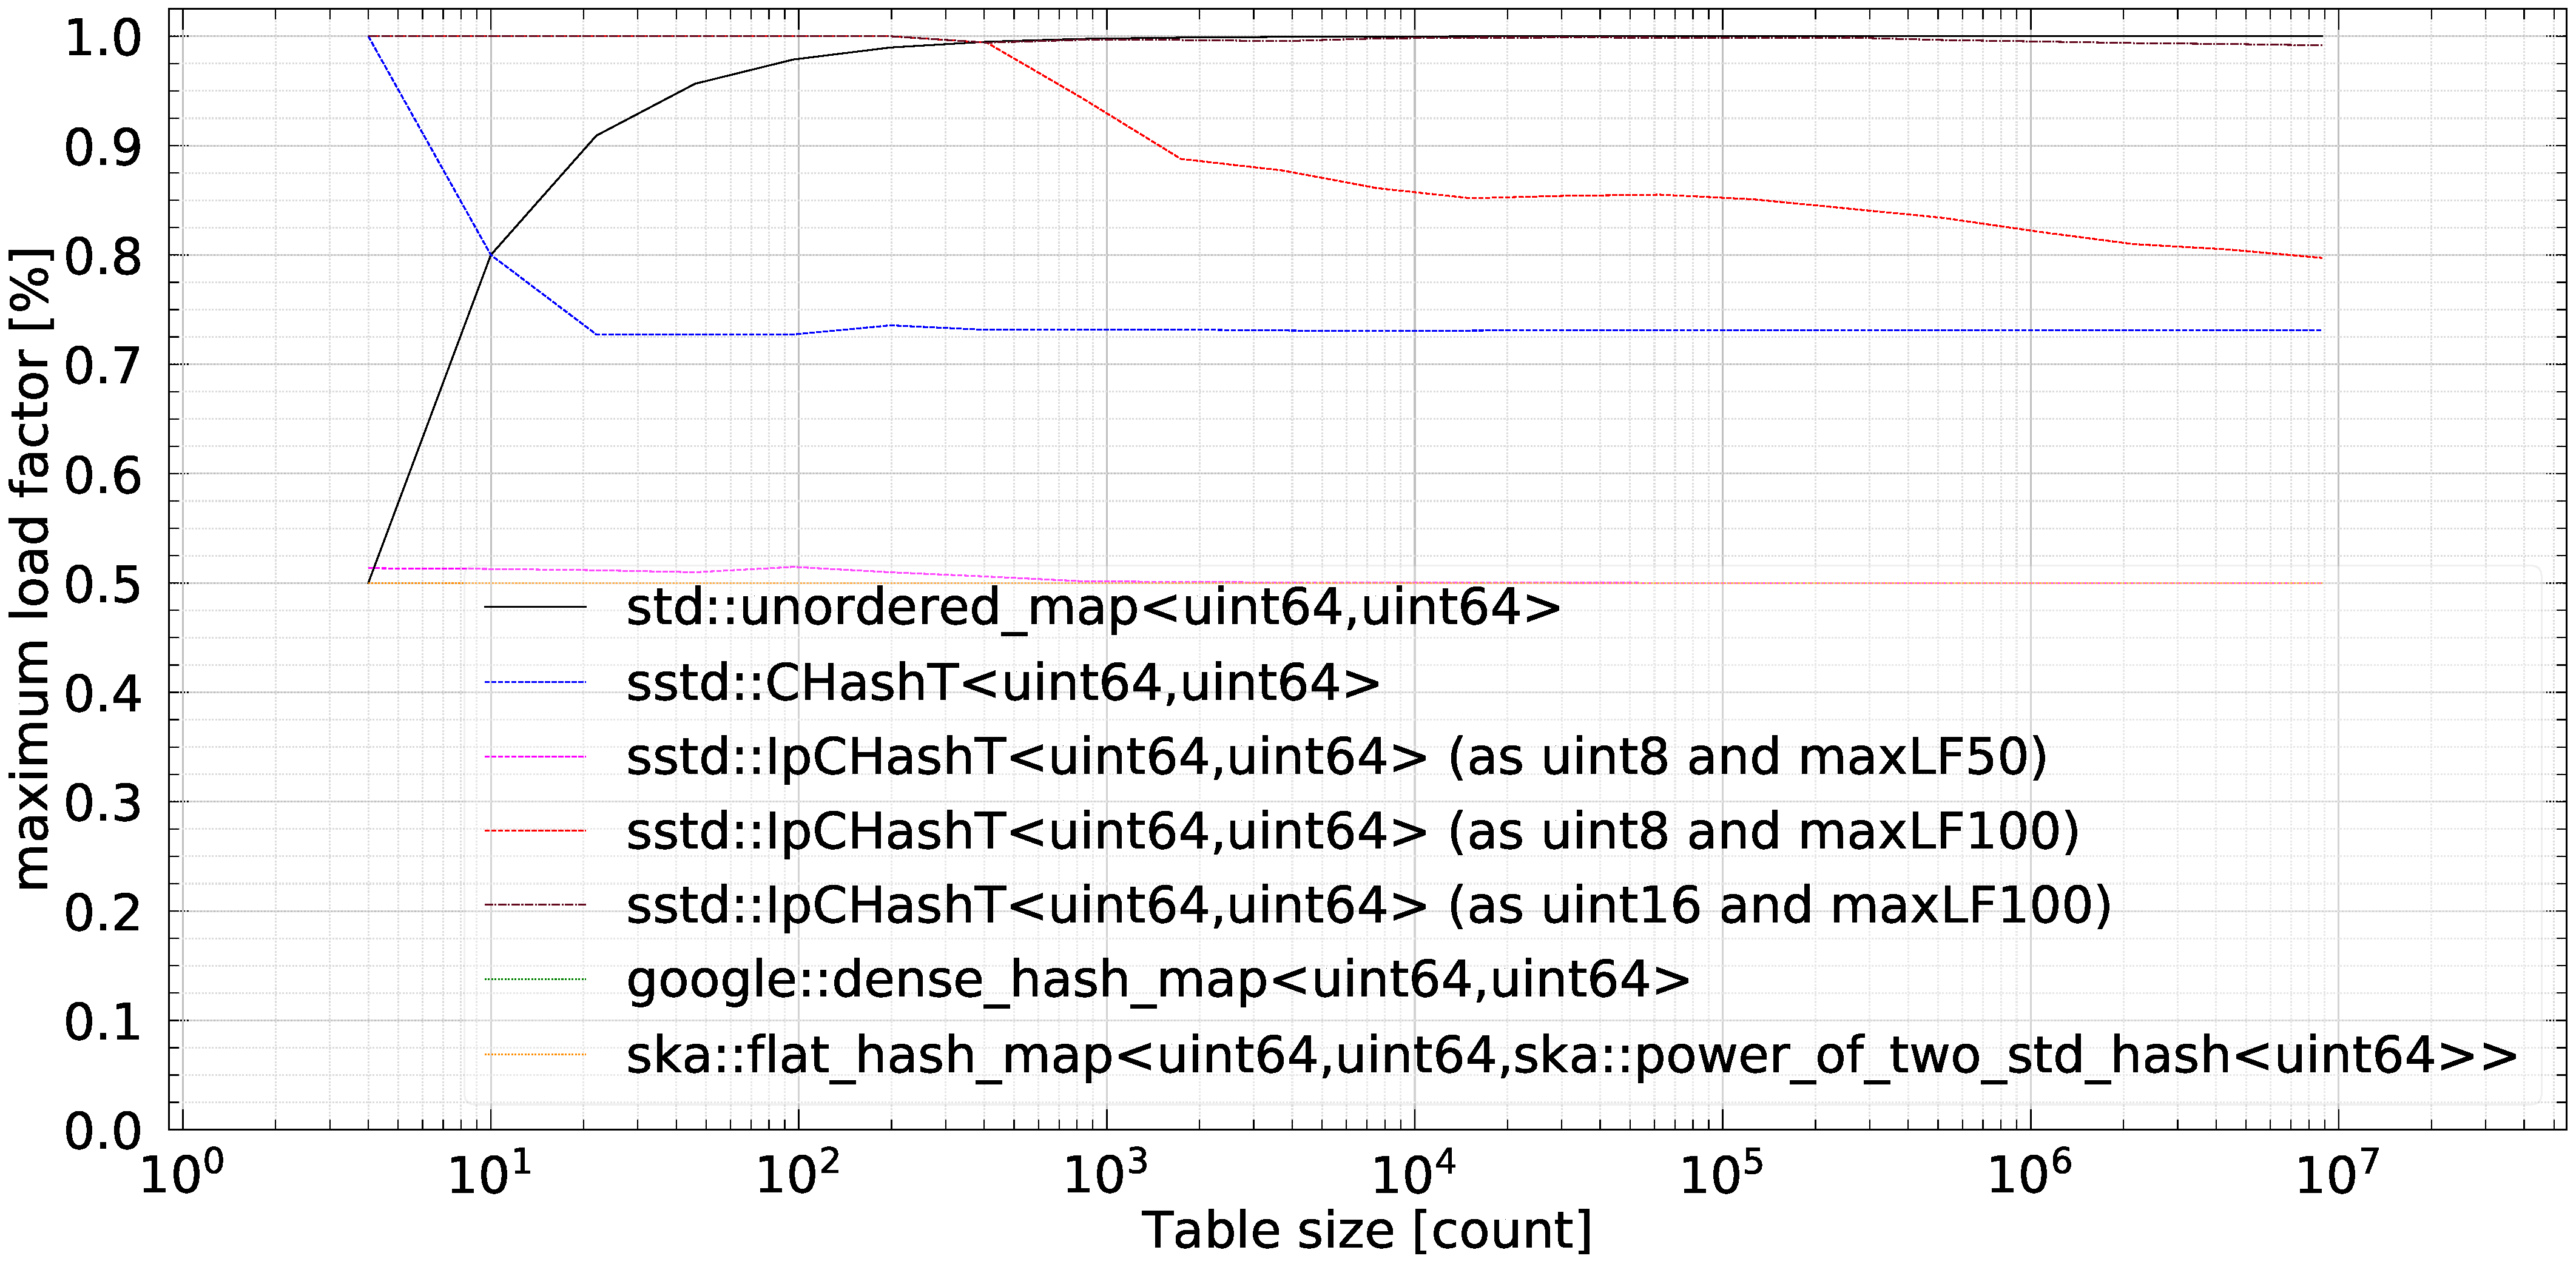
\includegraphics[scale=0.24]{./fig_bench/maxLoadFactor_med.pdf}
  \caption{
    Maximum load factor which is median value of 100 samples.
    Maximum load factor of IpHashT (uint16, maxLF100) is limitted by its maximum length of shift\_T.
    Maximum load factor of IpHashT (uint8, maxLF50), dense\_hash\_map and flat\_hash\_map is artificially limited by 50 \%.
  }
  \label{fig_bench_LF}
\end{figure}

%%%

\begin{figure}[]
%  \vspace{-5mm}
  \hspace{-1mm}
  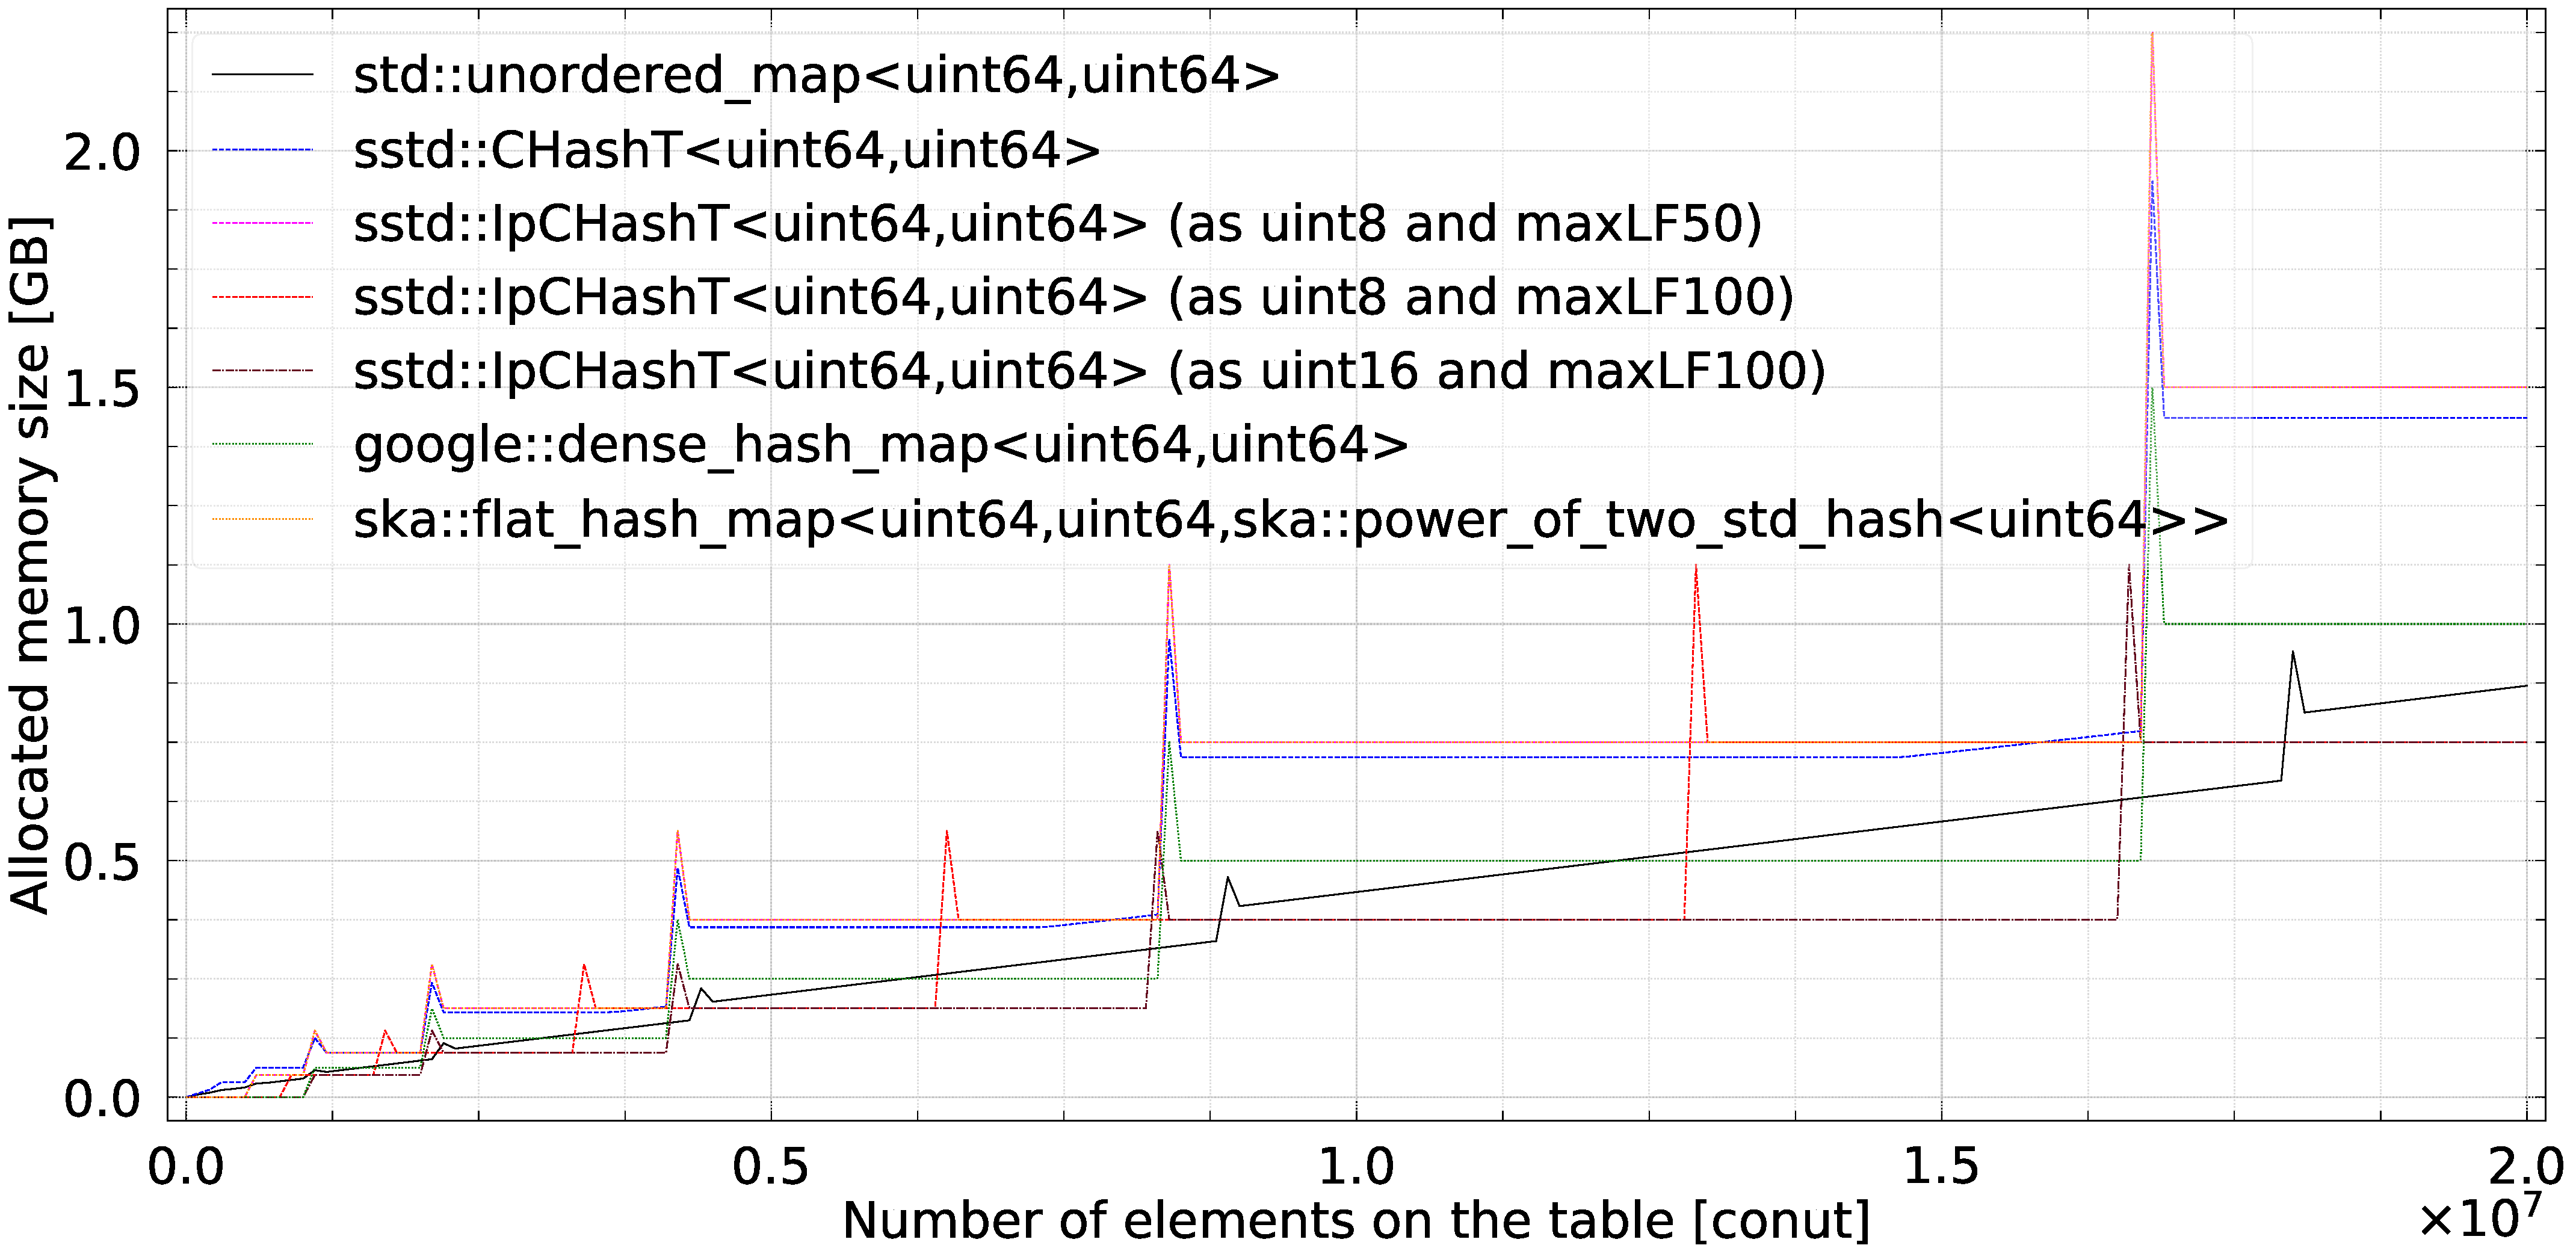
\includegraphics[scale=0.24]{./fig_bench/usedMemory.pdf}
  \caption{
    Allocated memory size, which is one sample raw data.
    Peaks of memory size indicate rehash timmings.
    And the width of peaks is measurement interval since the ture peak is as narrow as one step of x axis.
    unordered\_map seems to allocating memory each by insertion.
    IpCHashTs are moved the timming of rehashing back and forth by the influence of maximum load factor.
    flat\_hash\_map while it is hard to see, is plotted on the same place of IpCHashT (uint8, maxLF50).
  }
  \label{fig_bench_memory}
%  \vspace{-10mm}
\end{figure}

\begin{figure}[h]
%  \vspace{-5mm}
  \hspace{-1mm}
  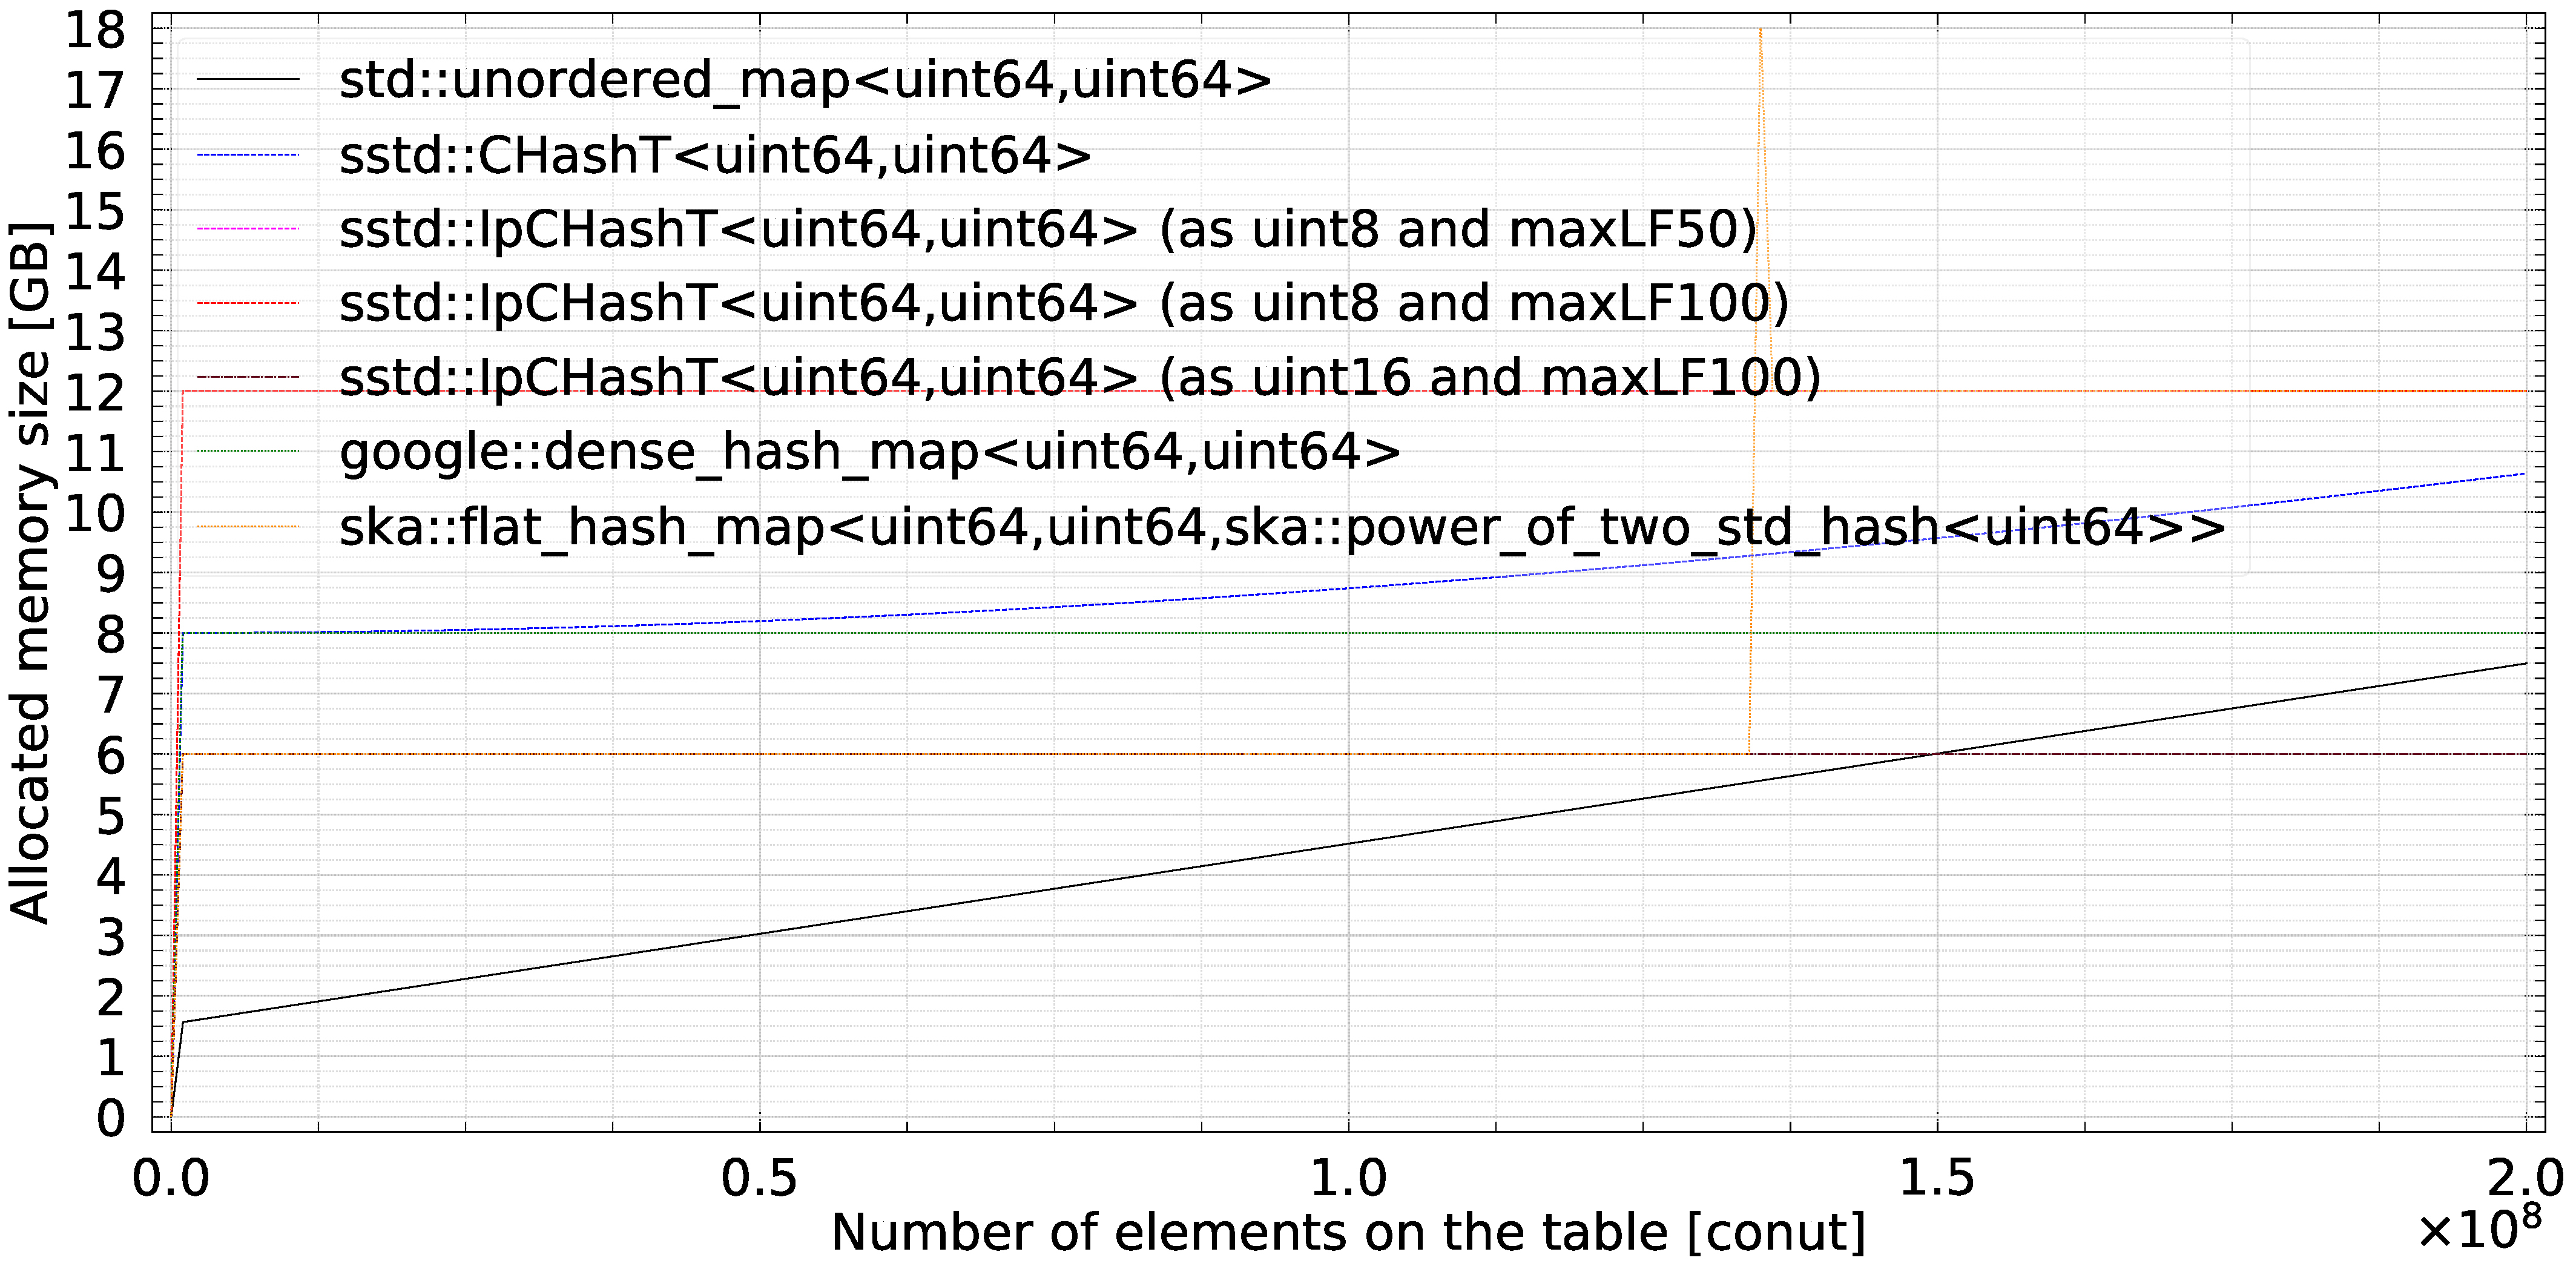
\includegraphics[scale=0.24]{./fig_bench/usedMemory_preAlloc.pdf}
  \caption{
    Allocated memory size, which is one sample raw data.
    In this measurement, each hash table is pre-allocated with $2.0\times10^8$.
%    Peak of memory size indicate rehash timmings.
%    And the width of peaks is measurement interval since the ture peak is as narrow as one step of x axis.
    IpCHashT (uint8, maxLF100), while it is hard to see, is plotted on the same place of IpCHashT (uint8, maxLF50).
    flat\_hash\_map is initializing its table size with $2.0\times10^8$ and the others are initializing their table size with $2.0\times10^8$ as a containable size.
    This means that the one with a rehashing peak is flat\_hash\_map.
  }
  \label{fig_bench_memory_preAlloc}
%  \vspace{-10mm}
\end{figure}

%%%

\begin{figure}[h]
  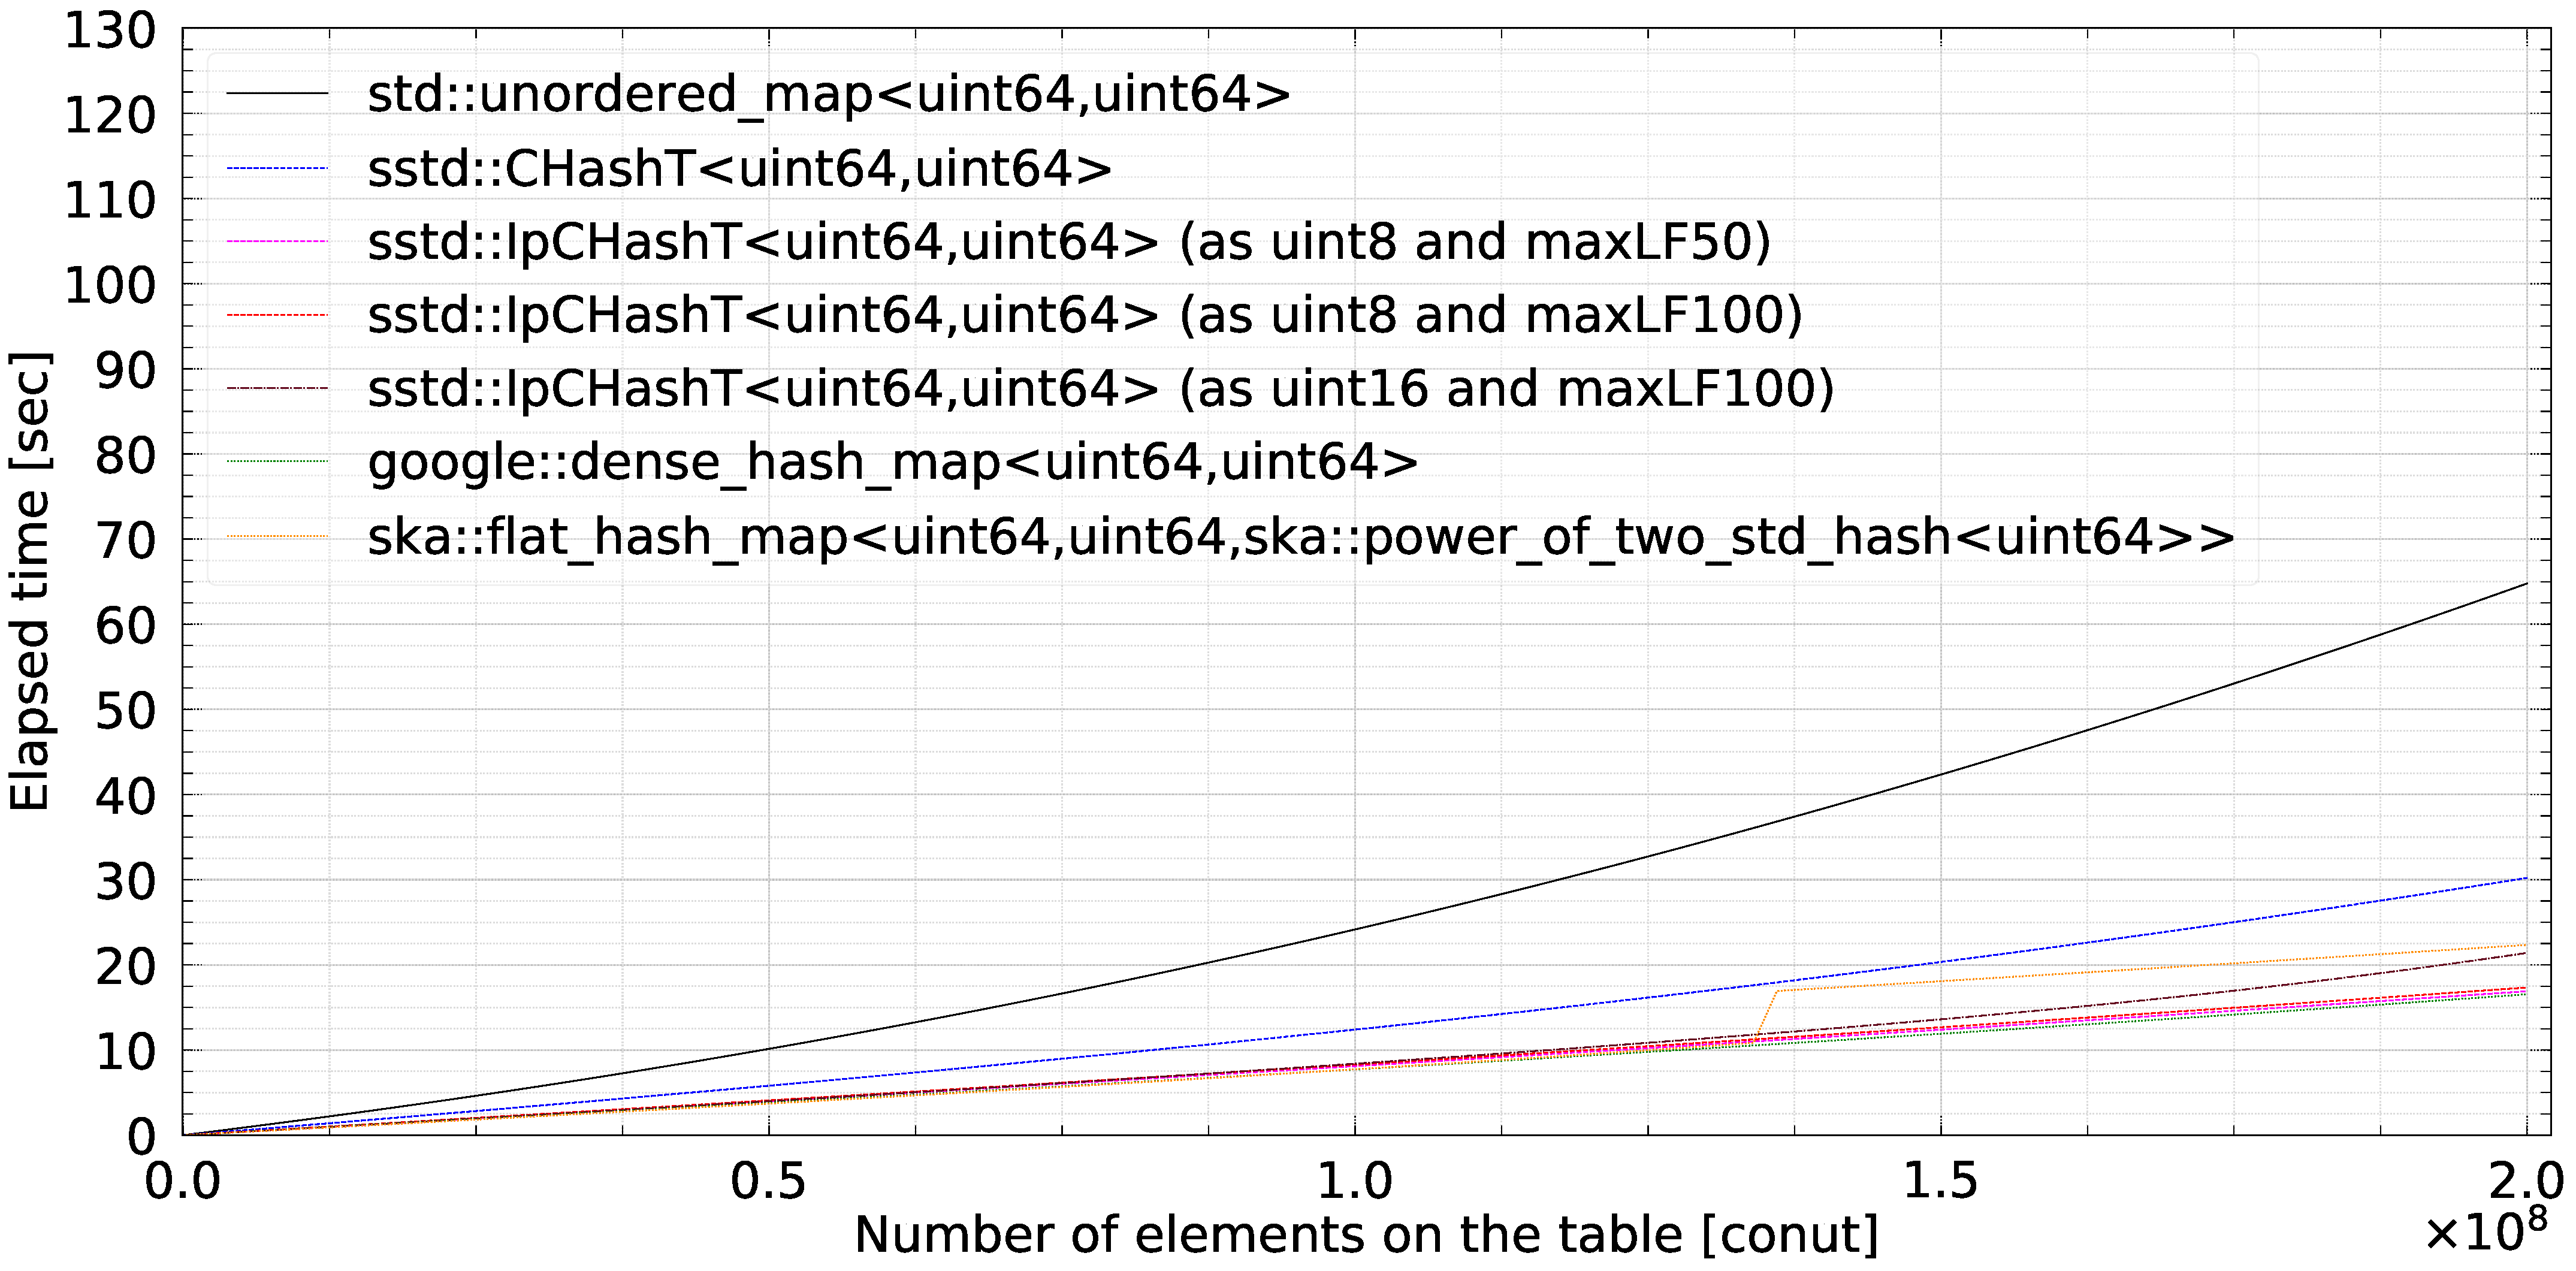
\includegraphics[scale=0.24]{./fig_bench/insert_et_preAlloc_med.pdf}
  \caption{
    Total time of insertion, which is a median value of 100 samples, using pre-allocated table.
    In this measurement, each hash table is pre-allocated with $2.0\times10^8$.
    A discontinuous value around $1.25\textasciitilde.375\times10^8$ represents rehashing of flat\_hash\_map.
    This is due to differences in the algorithms that determine the initial table size.
  }
  \label{fig_bench_insert_preAlloc}
\end{figure}

\begin{figure}[h]
  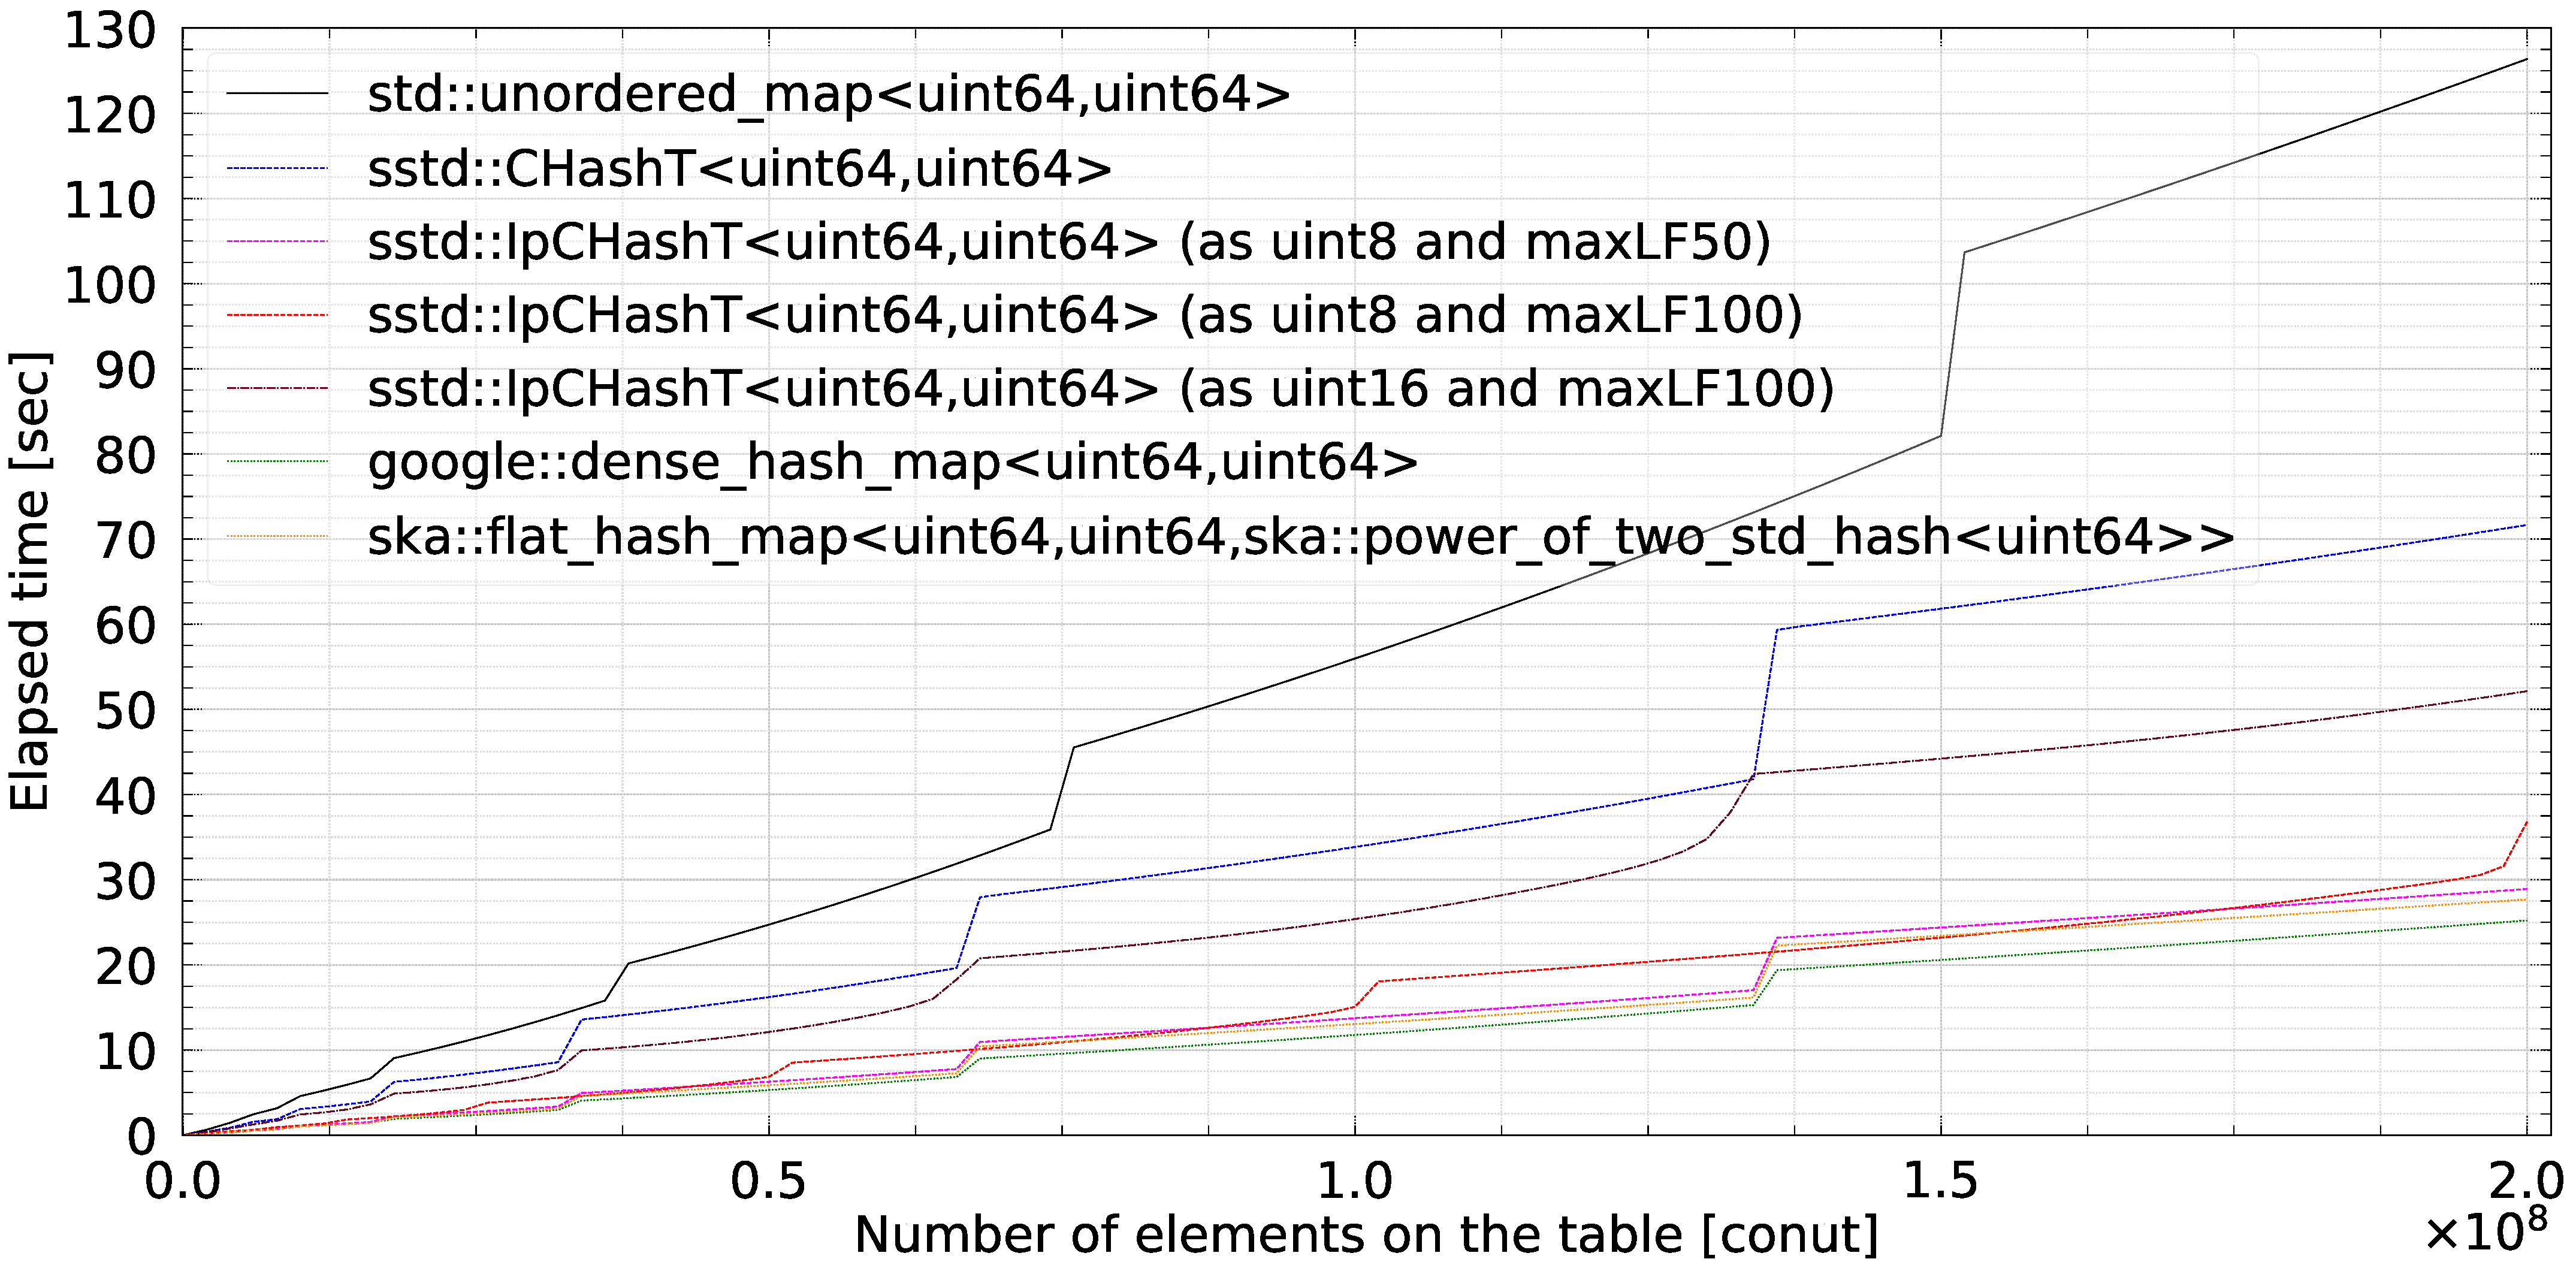
\includegraphics[scale=0.24]{./fig_bench/insert_et_med.pdf}
  \caption{
    Total time of insertion, which is a median value of 100 samples, with rehashing table.
    Chaining type of hash tables like, CHashT and IpCHashTs (especially uint16-maxLF100 option), are slow down its insertion speed as the load factor increase.
  }
  \label{fig_bench_insert_wRehash}
\end{figure}

\begin{figure}[h]
  \hspace{-3mm}
  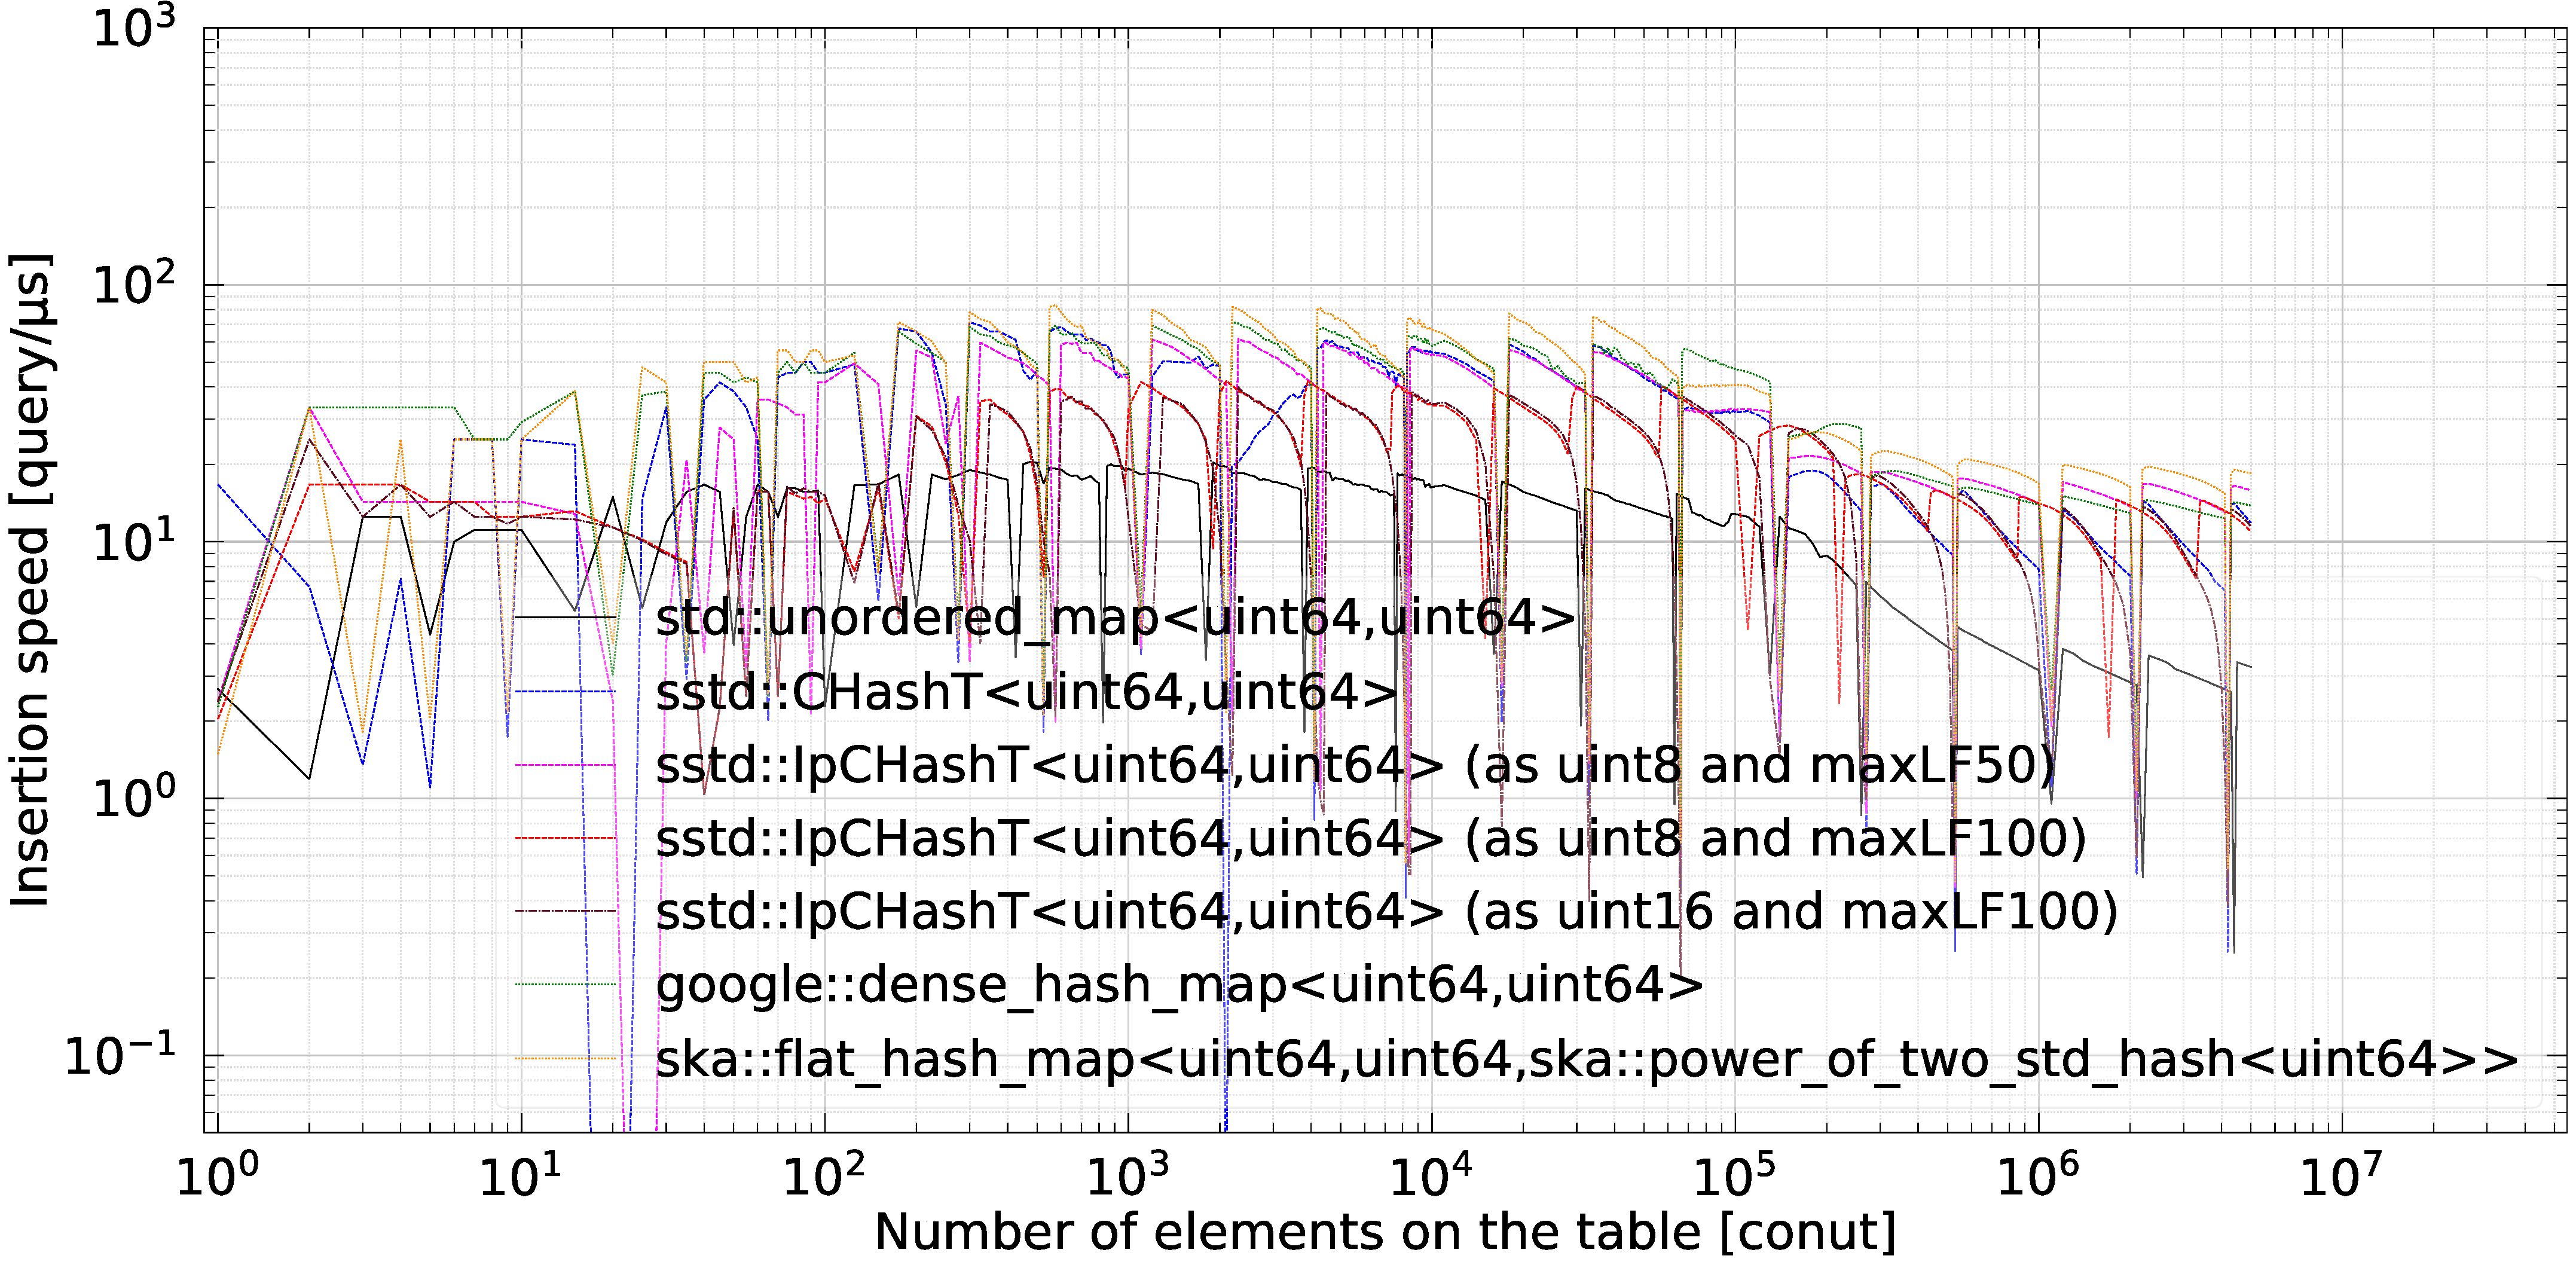
\includegraphics[scale=0.24]{./fig_bench/insert_med.pdf}
  \caption{
    Insertion speed, which is a median value of 100 samples.
    The spikes formed by the valleys represent rehashings.
    The CPU cache line is around $1.0\times10^5$ elements for 4 MB L2 cache and around $1.0\times10^6$ elements for 16 MB L3 cache on AMD Ryzen7 1700.
  }
  \label{fig_bench_insert}
\end{figure}

%%%

\begin{figure}[h]
  \hspace{-3mm}
  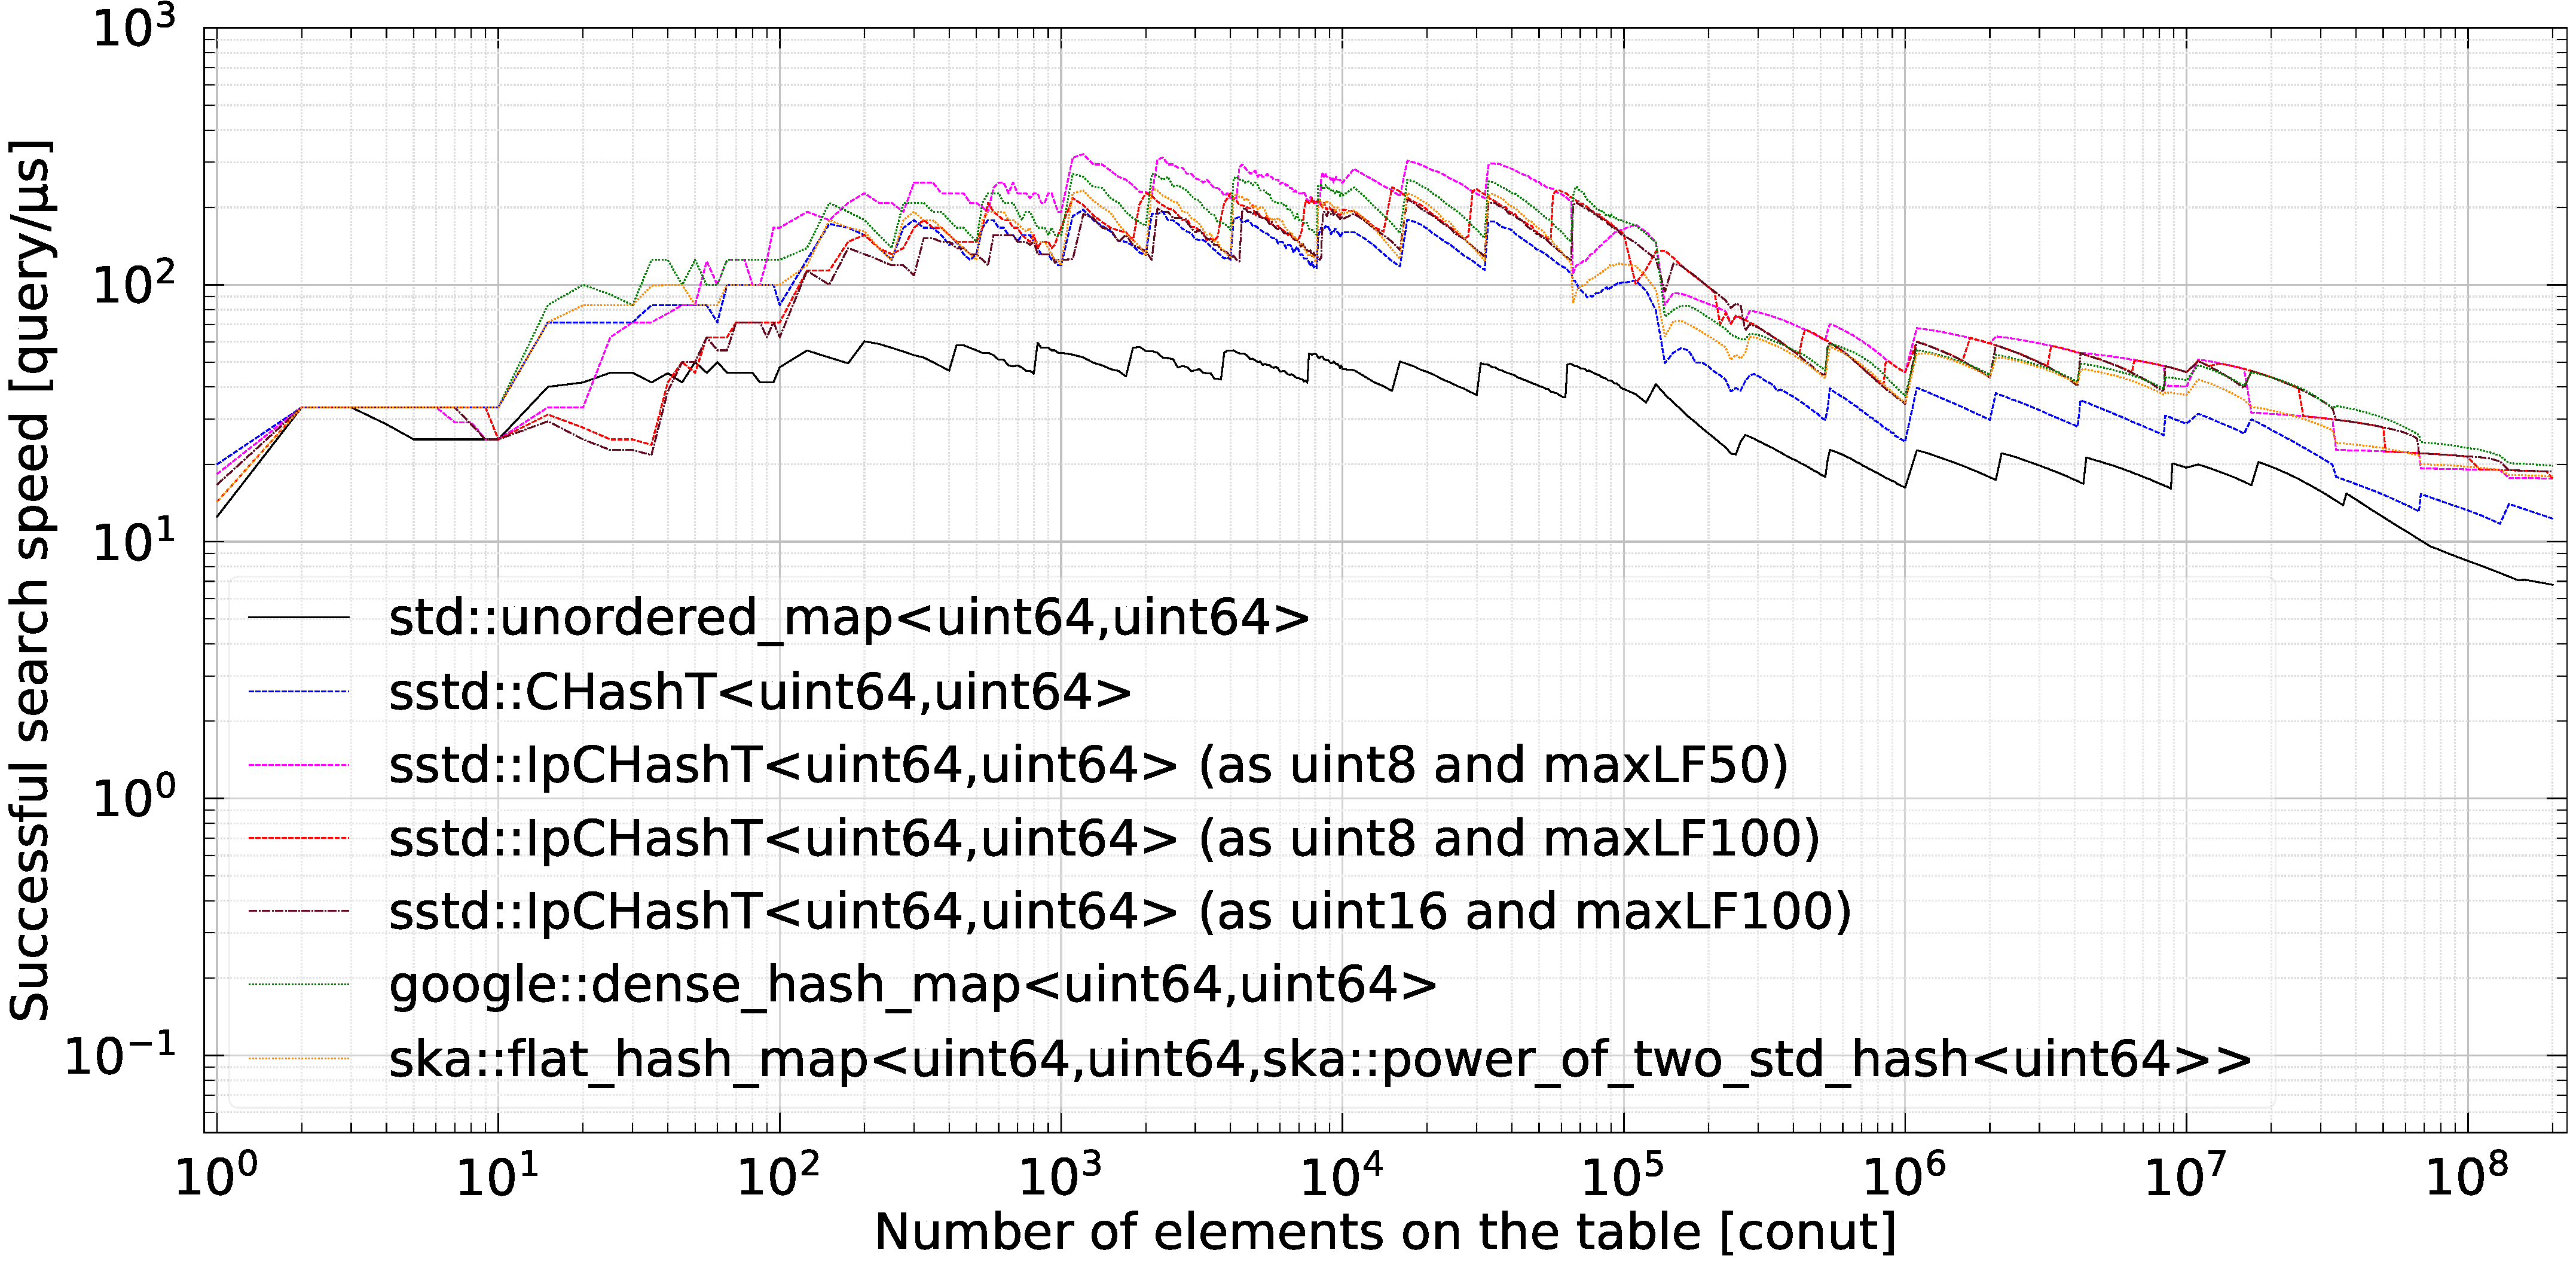
\includegraphics[scale=0.24]{./fig_bench_sm/find_successful_search_med.pdf}
  \caption{
    (Successful search major option). Successful search speed, which is a median value of 100 samples.
    About $1.0\times10^5$ elements will consume totally 4 MB of L2 cache,
    and about $1.0\times10^6$ elements will consume totally 16 MB of L3 cache on AMD Ryzen7 1700.
  }
  \label{fig_bench_find_s_sm}
\end{figure}

\begin{figure}[h]
  \hspace{-3mm}
  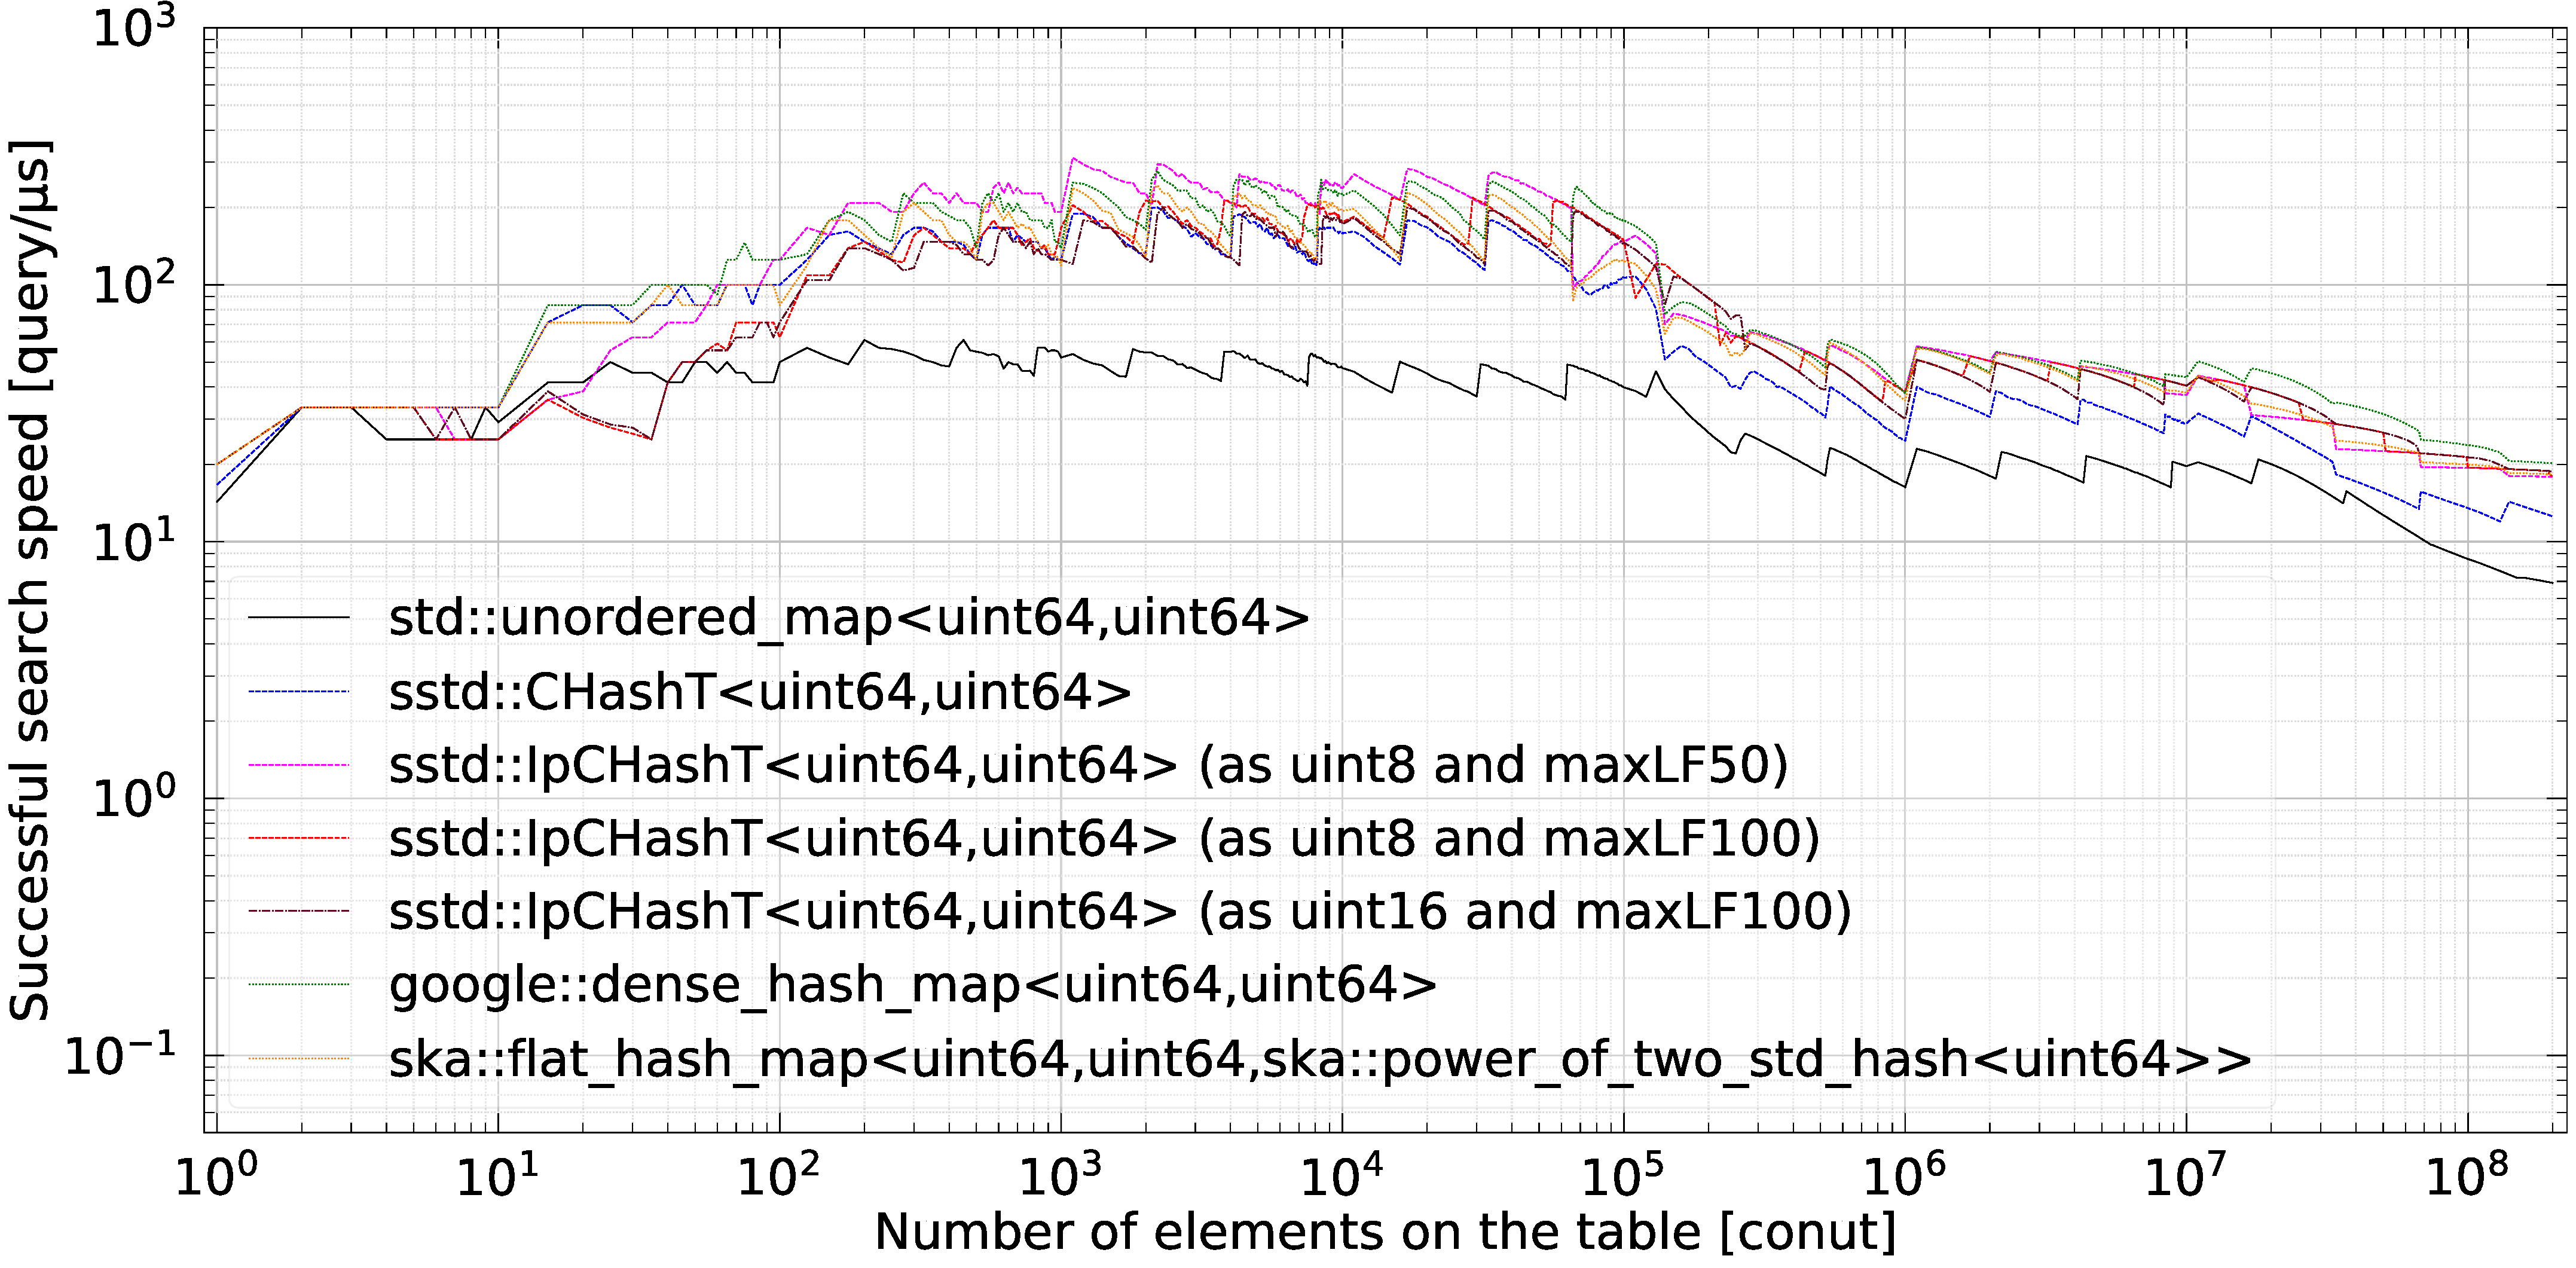
\includegraphics[scale=0.24]{./fig_bench_usm/find_successful_search_med.pdf}
  \caption{
    (Unsuccessful search major option). Successful search speed, which is a median value of 100 samples.
    About $1.0\times10^5$ elements will consume totally 4 MB of L2 cache,
    and about $1.0\times10^6$ elements will consume totally 16 MB of L3 cache on AMD Ryzen7 1700.
  }
  \label{fig_bench_find_s_um}
\end{figure}

%%%

\begin{figure}[h]
  \hspace{-3mm}
  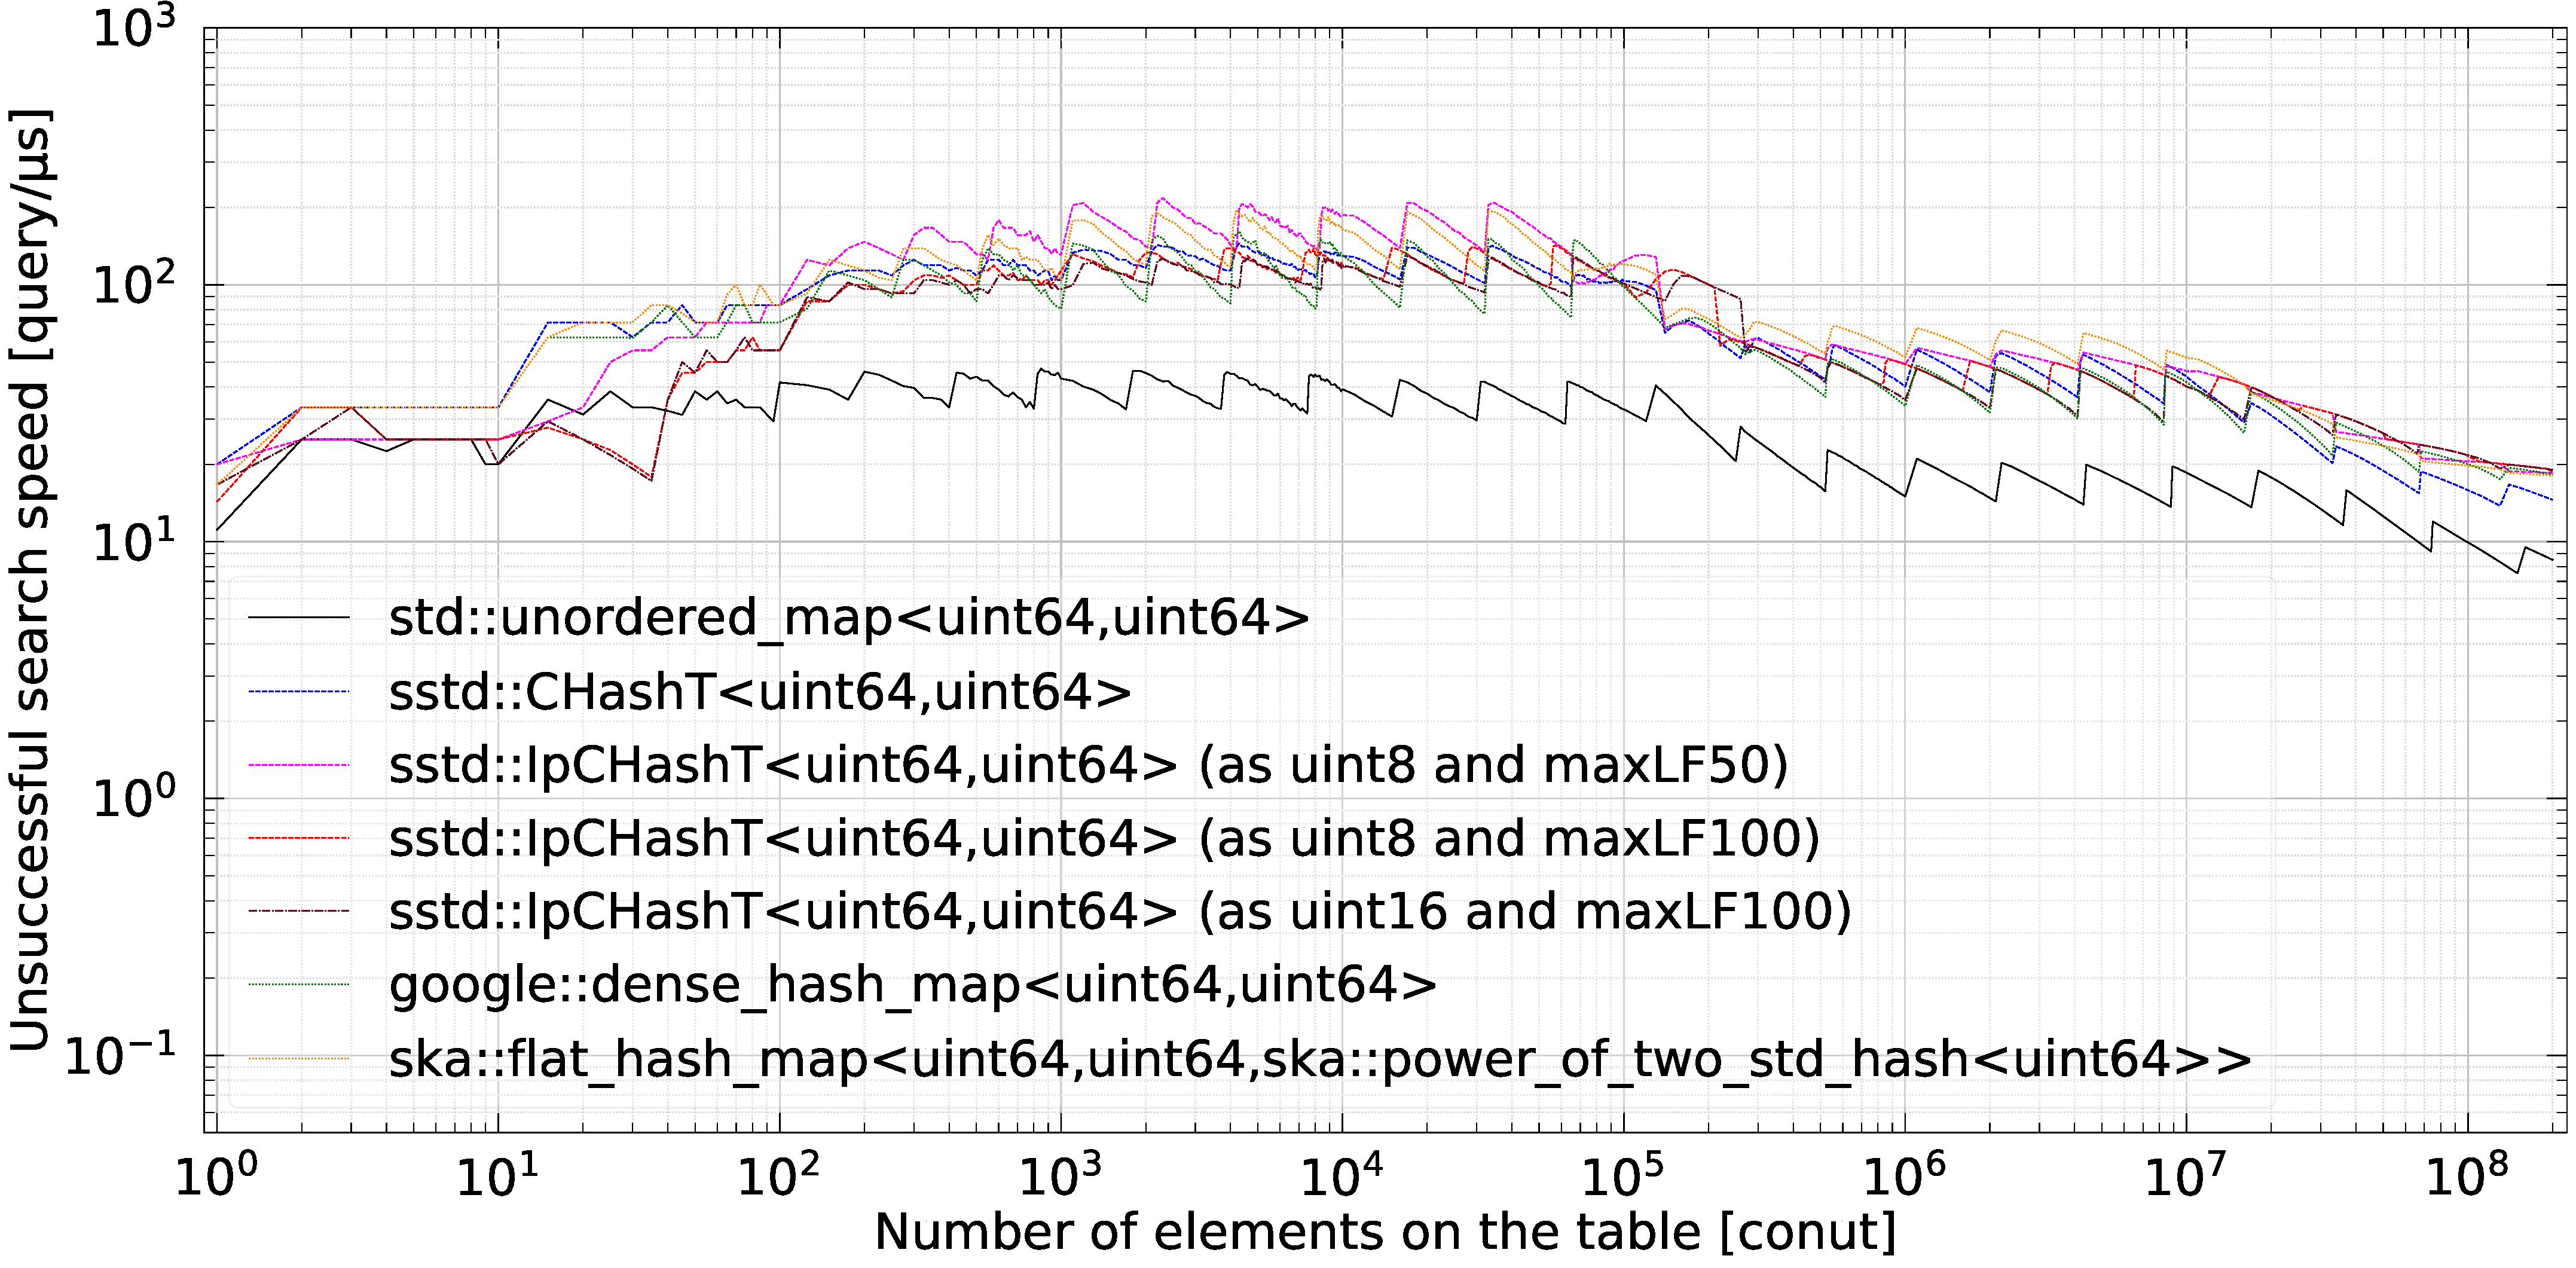
\includegraphics[scale=0.24]{./fig_bench_sm/find_unsuccessful_search_med.pdf}
  \caption{
    (Successful search major option). Unsuccessful search speed, which is a median value of 100 samples.
    About $1.0\times10^5$ elements will consume totally 4 MB of L2 cache,
    and about $1.0\times10^6$ elements will consume totally 16 MB of L3 cache on AMD Ryzen7 1700.
  }
  \label{fig_bench_find_us_sm}
\end{figure}

\begin{figure}[h]
  \hspace{-3mm}
  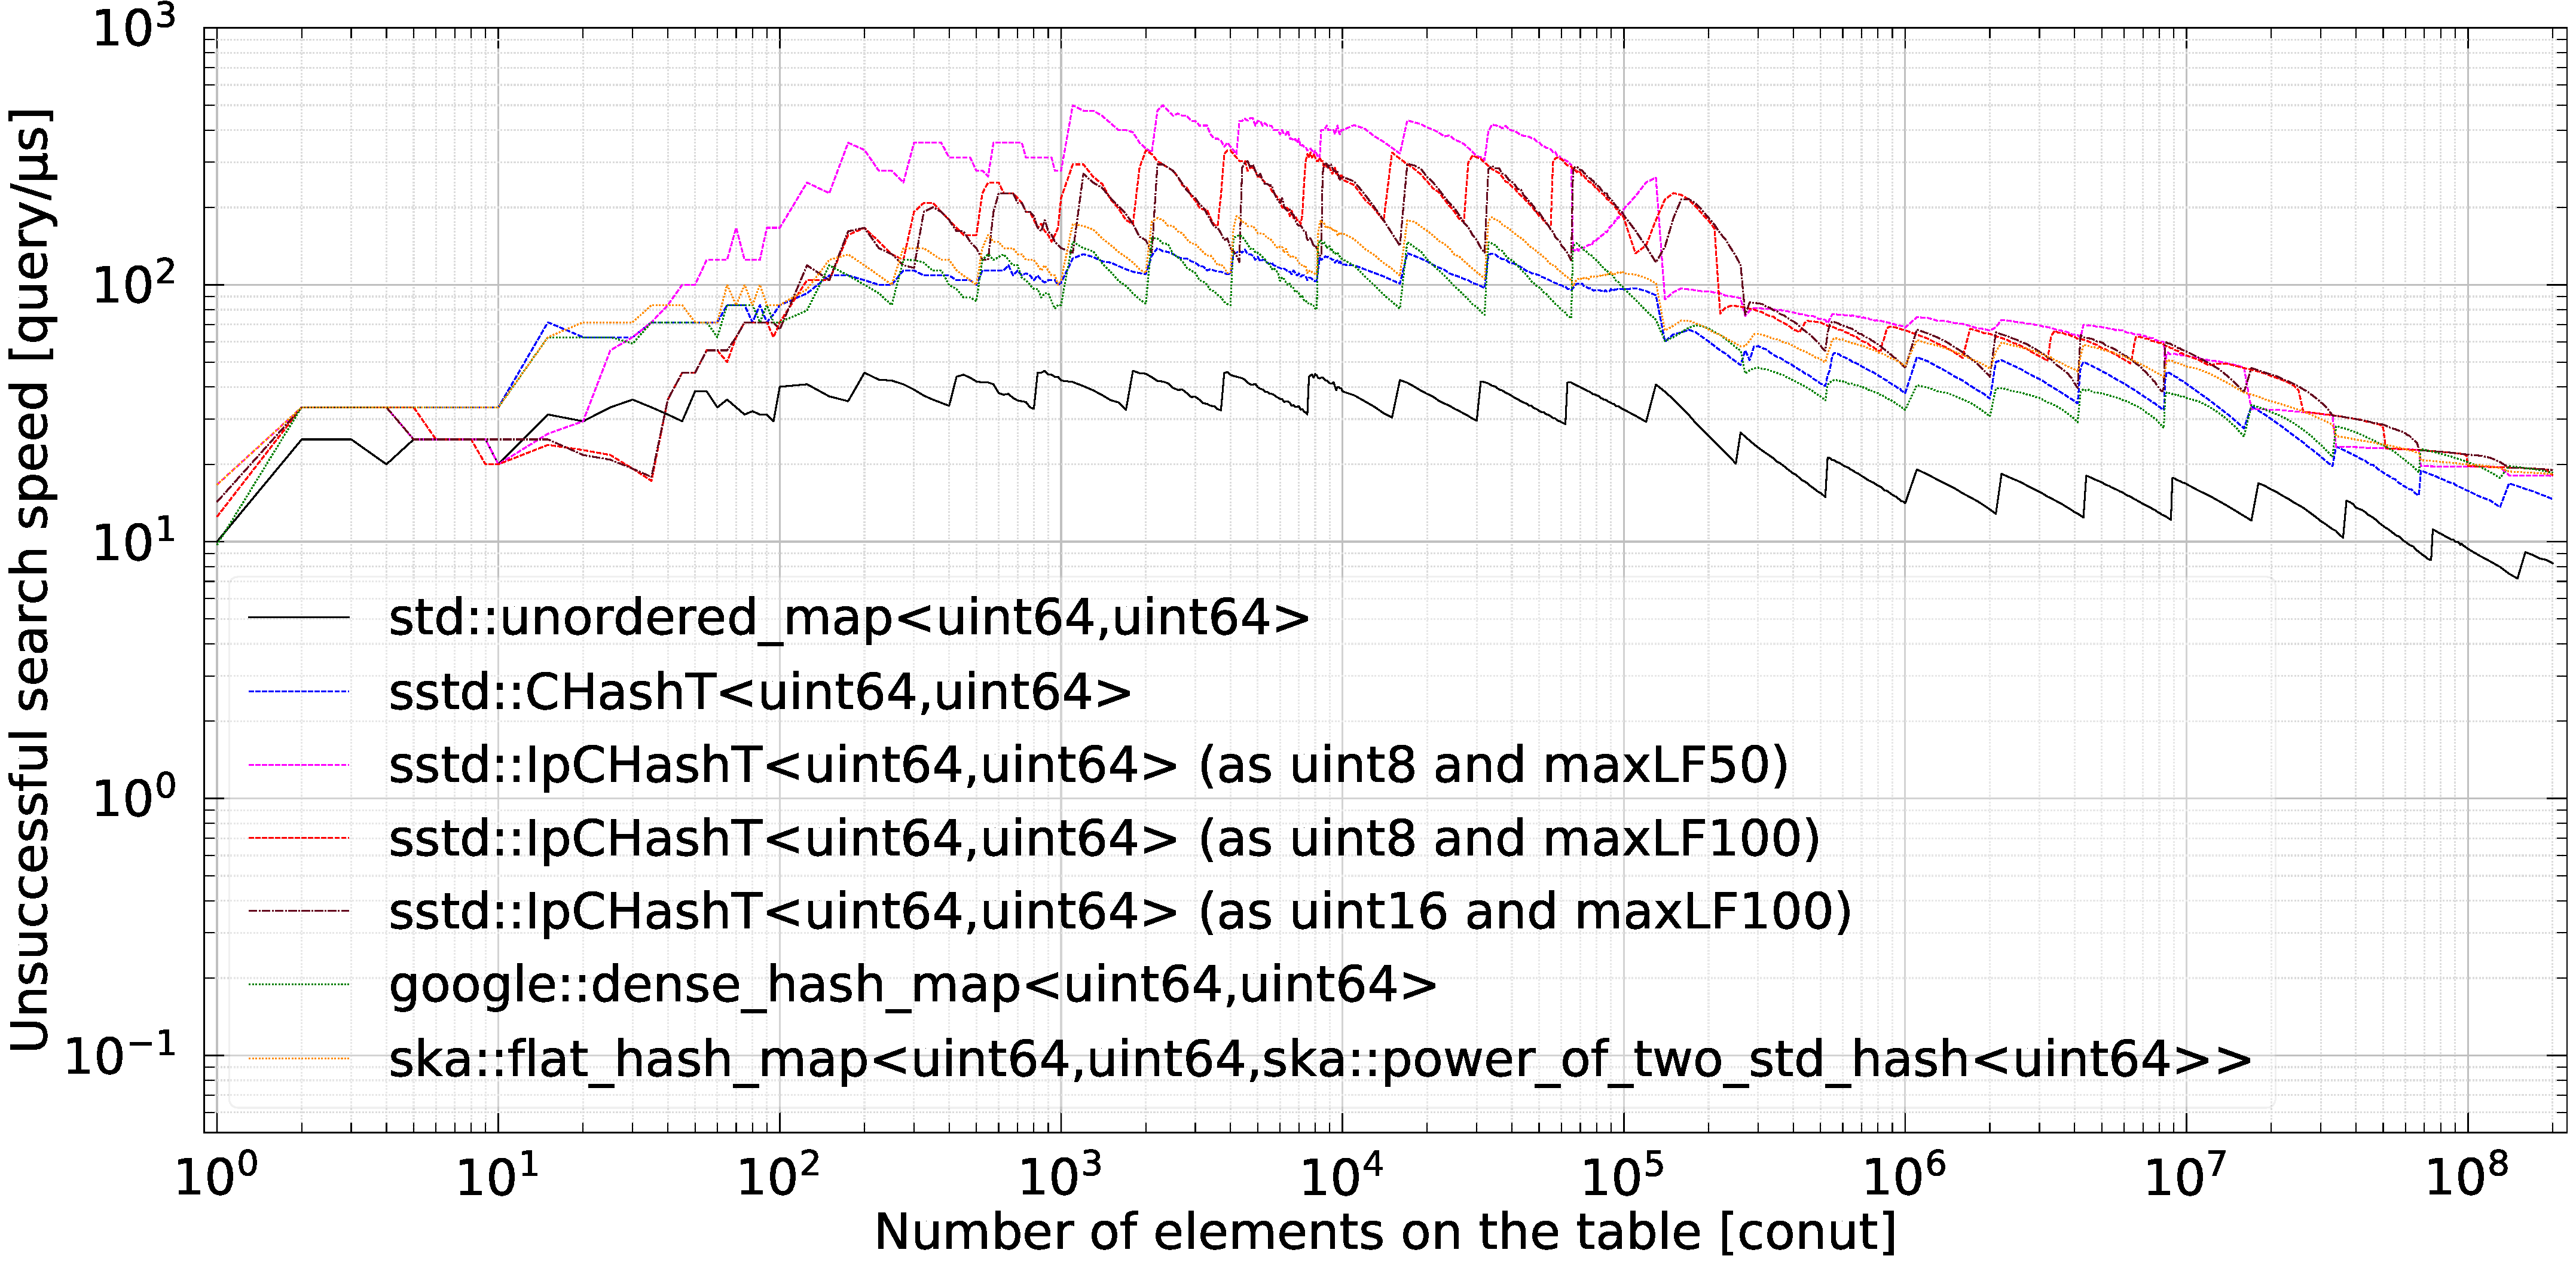
\includegraphics[scale=0.24]{./fig_bench_usm/find_unsuccessful_search_med.pdf}
  \caption{
    (Unsuccessful search major option). Unsuccessful search speed, which is a median value of 100 samples.
    About $1.0\times10^5$ elements will consume totally 4 MB of L2 cache,
    and about $1.0\times10^6$ elements will consume totally 16 MB of L3 cache on AMD Ryzen7 1700.
  }
  \label{fig_bench_find_us_um}
\end{figure}

%%%

\begin{figure}[h]
  \hspace{-3mm}
  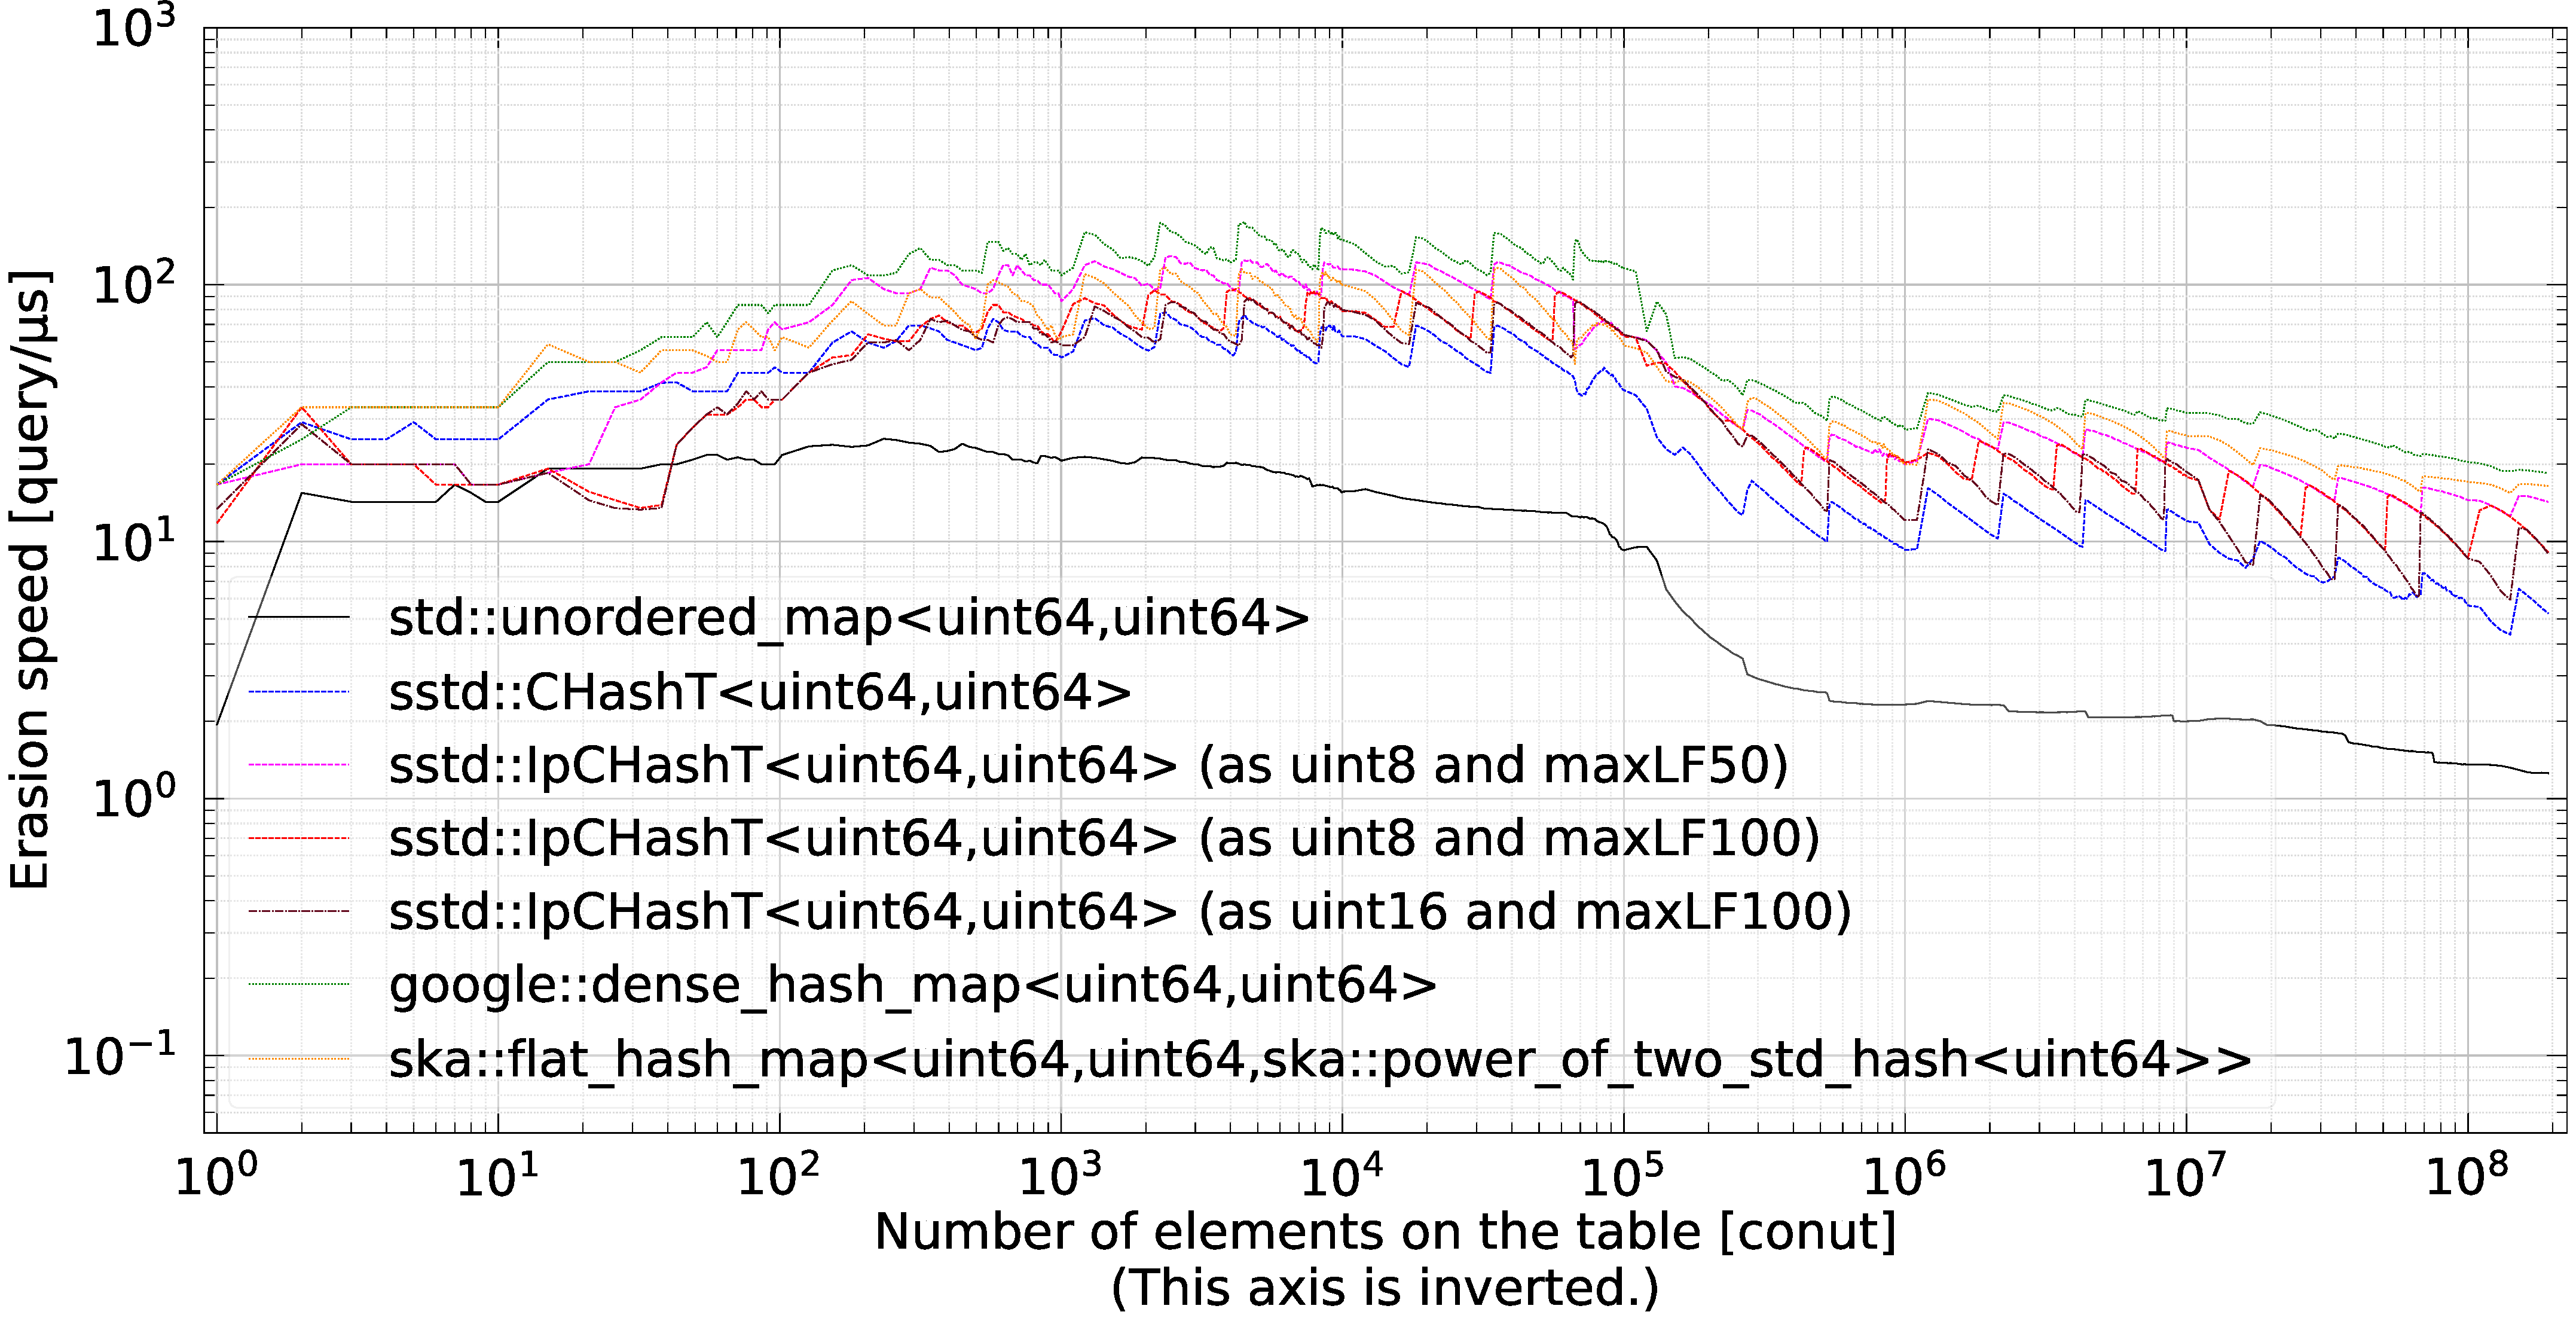
\includegraphics[scale=0.24]{./fig_bench_sm/erase_med.pdf}
  \caption{
    (Successful search major option). Erasion speed, which is a median value of 100 samples.
    About $1.0\times10^5$ elements will consume totally 4 MB of L2 cache,
    and about $1.0\times10^6$ elements will consume totally 16 MB of L3 cache on AMD Ryzen7 1700.
  }
  \label{fig_bench_erase_sm}
\end{figure}

\begin{figure}[h]
  \hspace{-3mm}
  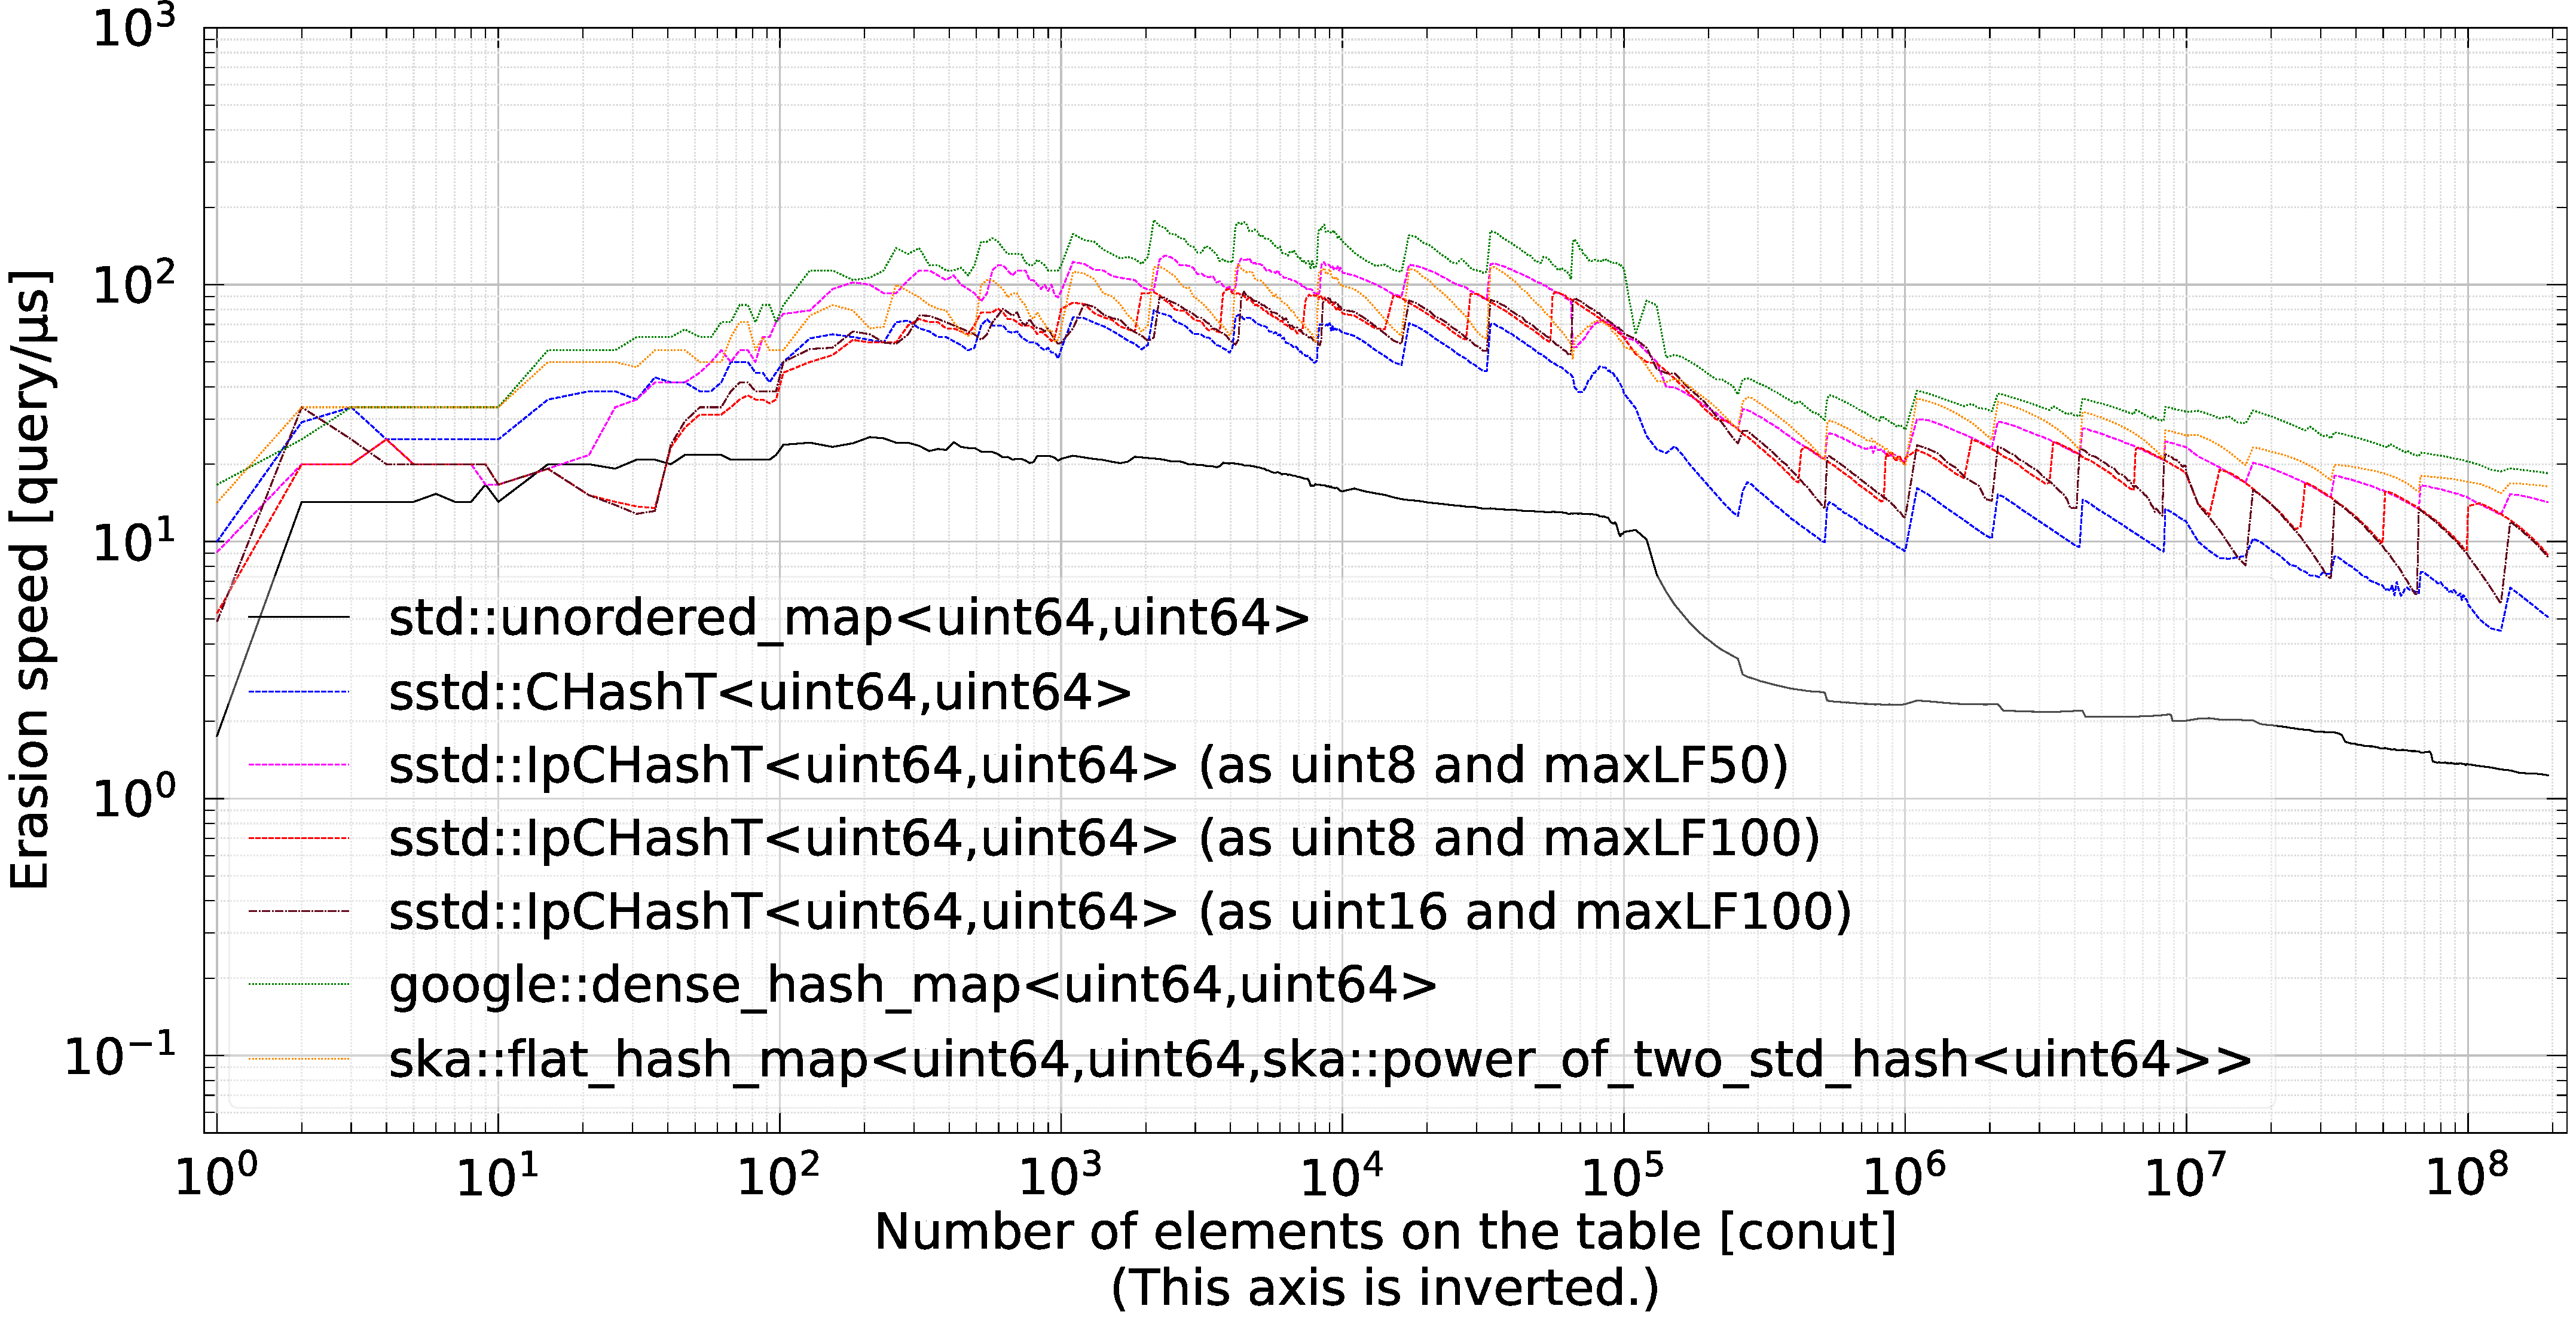
\includegraphics[scale=0.24]{./fig_bench_usm/erase_med.pdf}
  \caption{
    (Unsuccessful search major option). Erasion speed, which is a median value of 100 samples.
    About $1.0\times10^5$ elements will consume totally 4 MB of L2 cache,
    and about $1.0\times10^6$ elements will consume totally 16 MB of L3 cache on AMD Ryzen7 1700.
  }
  \label{fig_bench_erase_um}
\end{figure}

%%%%%%%%%%%%%%%%%%%%%%%%%%%%%%%%%%%%%%%%%%%%%%%%%%%%%%%%%%%%%%%%%%%%%%%%%%%%%%%%%%%%%%%%%%%%%%%%%%%%%%%%%%%%%%%%%%%%%%%%%%%%%%%%%%%%%%%%%%%%%%%%%















